% !TEX program = pdflatex
\documentclass[letterpaper,12pt]{article}
\usepackage[spanish,mexico]{babel}
\usepackage[T1]{fontenc}
\usepackage{lmodern}
\usepackage{amsmath,amssymb}
\usepackage{graphicx,float,subcaption,xcolor,array,booktabs,tabularx,ragged2e}
\usepackage{tikz}
\usetikzlibrary{arrows.meta,positioning,shapes.geometric,calc}
\usepackage{listings}
\usepackage[left=25mm,right=25mm,top=35mm,bottom=30mm,headheight=15pt]{geometry}
\usepackage{parskip,fancyhdr}
\usepackage{hyperref}

\graphicspath{{img/}{portada_img/}}
\newcommand{\materia}{Laboratorio de Organización y Arquitectura de Computadoras}
\pagestyle{fancy}
\fancyhf{}
\fancyhead[R]{\textsc{\materia}}
\fancyfoot[C]{\thepage}
\renewcommand{\headrulewidth}{0.8pt}
\hypersetup{colorlinks=true,linkcolor=blue,urlcolor=cyan}

\definecolor{codebg}{rgb}{0.96,0.96,0.96}
\definecolor{keyword}{rgb}{0.0,0.2,0.6}
\definecolor{comment}{rgb}{0.25,0.5,0.35}
\definecolor{codegray}{rgb}{0.5,0.5,0.5}
\definecolor{amber}{RGB}{255,191,0}
\lstdefinestyle{estiloVHDL}{
  language=VHDL,basicstyle=\ttfamily\scriptsize,
  backgroundcolor=\color{codebg},commentstyle=\color{comment}\itshape,
  keywordstyle=\color{keyword}\bfseries,numbers=left,
  numberstyle=\tiny\color{codegray},frame=single,breaklines=true,
  literate={á}{{\'a}}1 {é}{{\'e}}1 {í}{{\'i}}1 {ó}{{\'o}}1 {ú}{{\'u}}1 {ñ}{{\~n}}1,
  keepspaces=true,showstringspaces=false,tabsize=4,
  morekeywords={library,use,all,entity,is,port,in,out,architecture,of,begin,end,signal,constant,process,if,then,else,elsif,case,when,others,std_logic,std_logic_vector}
}

\begin{document}
\thispagestyle{empty} % Sin encabezado ni pie en la portada

% --- ENCABEZADO DE PORTADA (TABLA DE 3 COLUMNAS) ---
\begin{center}
    % La tabla usa 'm' para centrar verticalmente las imágenes y el texto
    \begin{tabular}{m{0.15\textwidth} m{0.60\textwidth} m{0.15\textwidth}}
        % Logo Izquierdo (UNAM)
        
\includegraphics[width=2cm]{portada_img/escudounam_negro.jpg} & 
        
        % Título Central
        \centering\Huge\textbf{Universidad Nacional Autónoma de México} &
        
        % Logo Derecho (Facultad)
        \raggedleft
\includegraphics[width=2cm]{portada_img/escudofi_negro.jpg}
    \end{tabular}
\end{center}

\vspace{0.3cm}

% --- INFORMACIÓN DEL REPORTE ---
\begin{center}
    {\LARGE \textbf{Facultad de Ingeniería}}\\[1cm]

    {\LARGE \textbf{Laboratorio de Arquitectura y Organización de Computadoras}} \\[1cm]

	{\LARGE Grupo: 07 - Semestre: 2027-1} \\[1cm]
    
    {\LARGE \textbf{Reporte Práctica 6}}\\[0.5cm]
    {\LARGE {Secuenciador básico de 4 microinstrucciones}}\\[1cm]

    {\Large \textbf{Fecha de Entrega}}\\[0.2cm]
    {\Large 16 de Octubre del 2026} \\[1cm]

    {\LARGE \textbf{Profesor}}\\[0.2cm]
    {\Large Ing. Julio Cesar Cruz Estrada}\\[1cm]
    
    {\LARGE \textbf{Integrantes:}}\\[0.2cm]
    {\Large Espinoza Matamoros Percival Ulises}\\[0.5cm]
    {\Large Montiel Juárez Oscar Iván}\\[0.5cm]
    {\Large Veraza García Amy Valentina}\\[0.5cm]

\end{center}

\newpage

\section{Objetivo}

Familiarizar al alumno en el conocimiento del secuenciador básico, el cual es una parte fundamental del procesador.

\section{Desarrollo}

Un secuenciador es el bloque encargado de generar la dirección de la siguiente microinstrucción. En una unidad de control microprogramada, el registro $mPC$ contiene la dirección actual de la memoria de control. A partir de ella, el secuenciador puede continuar con la dirección consecutiva, cargar una liga asociada a un salto condicional, utilizar una dirección de transformación o atender una interrupción.

Para esta práctica se seleccionó la alternativa de cuatro microinstrucciones. El diseño se realizó con un contador de microprograma de cuatro bits, un incrementador, tres registros que entregan direcciones fijas y un multiplexor de cuatro entradas. La lógica interna recibe los bits $I_1I_0$ de la microinstrucción y la condición de control $CC$, con lo que genera los dos bits de selección del multiplexor.

\subsection{Microinstrucciones del secuenciador}

El esquema de referencia del profesor considera una ROM que entrega los campos de prueba, valor de prueba, tipo de microinstrucción, liga y salidas. En esta alternativa se implementó directamente el mecanismo de selección. Para probarlo, se aplicaron $I_1$, $I_0$ y $CC$ como entradas externas; los registros de liga, transformación e interrupción representan las direcciones almacenadas que normalmente provendrían de los campos correspondientes. La Figura~\ref{fig:secuenciador-general} muestra la conexión construida para este propósito.

\begin{figure}[H]
\centering
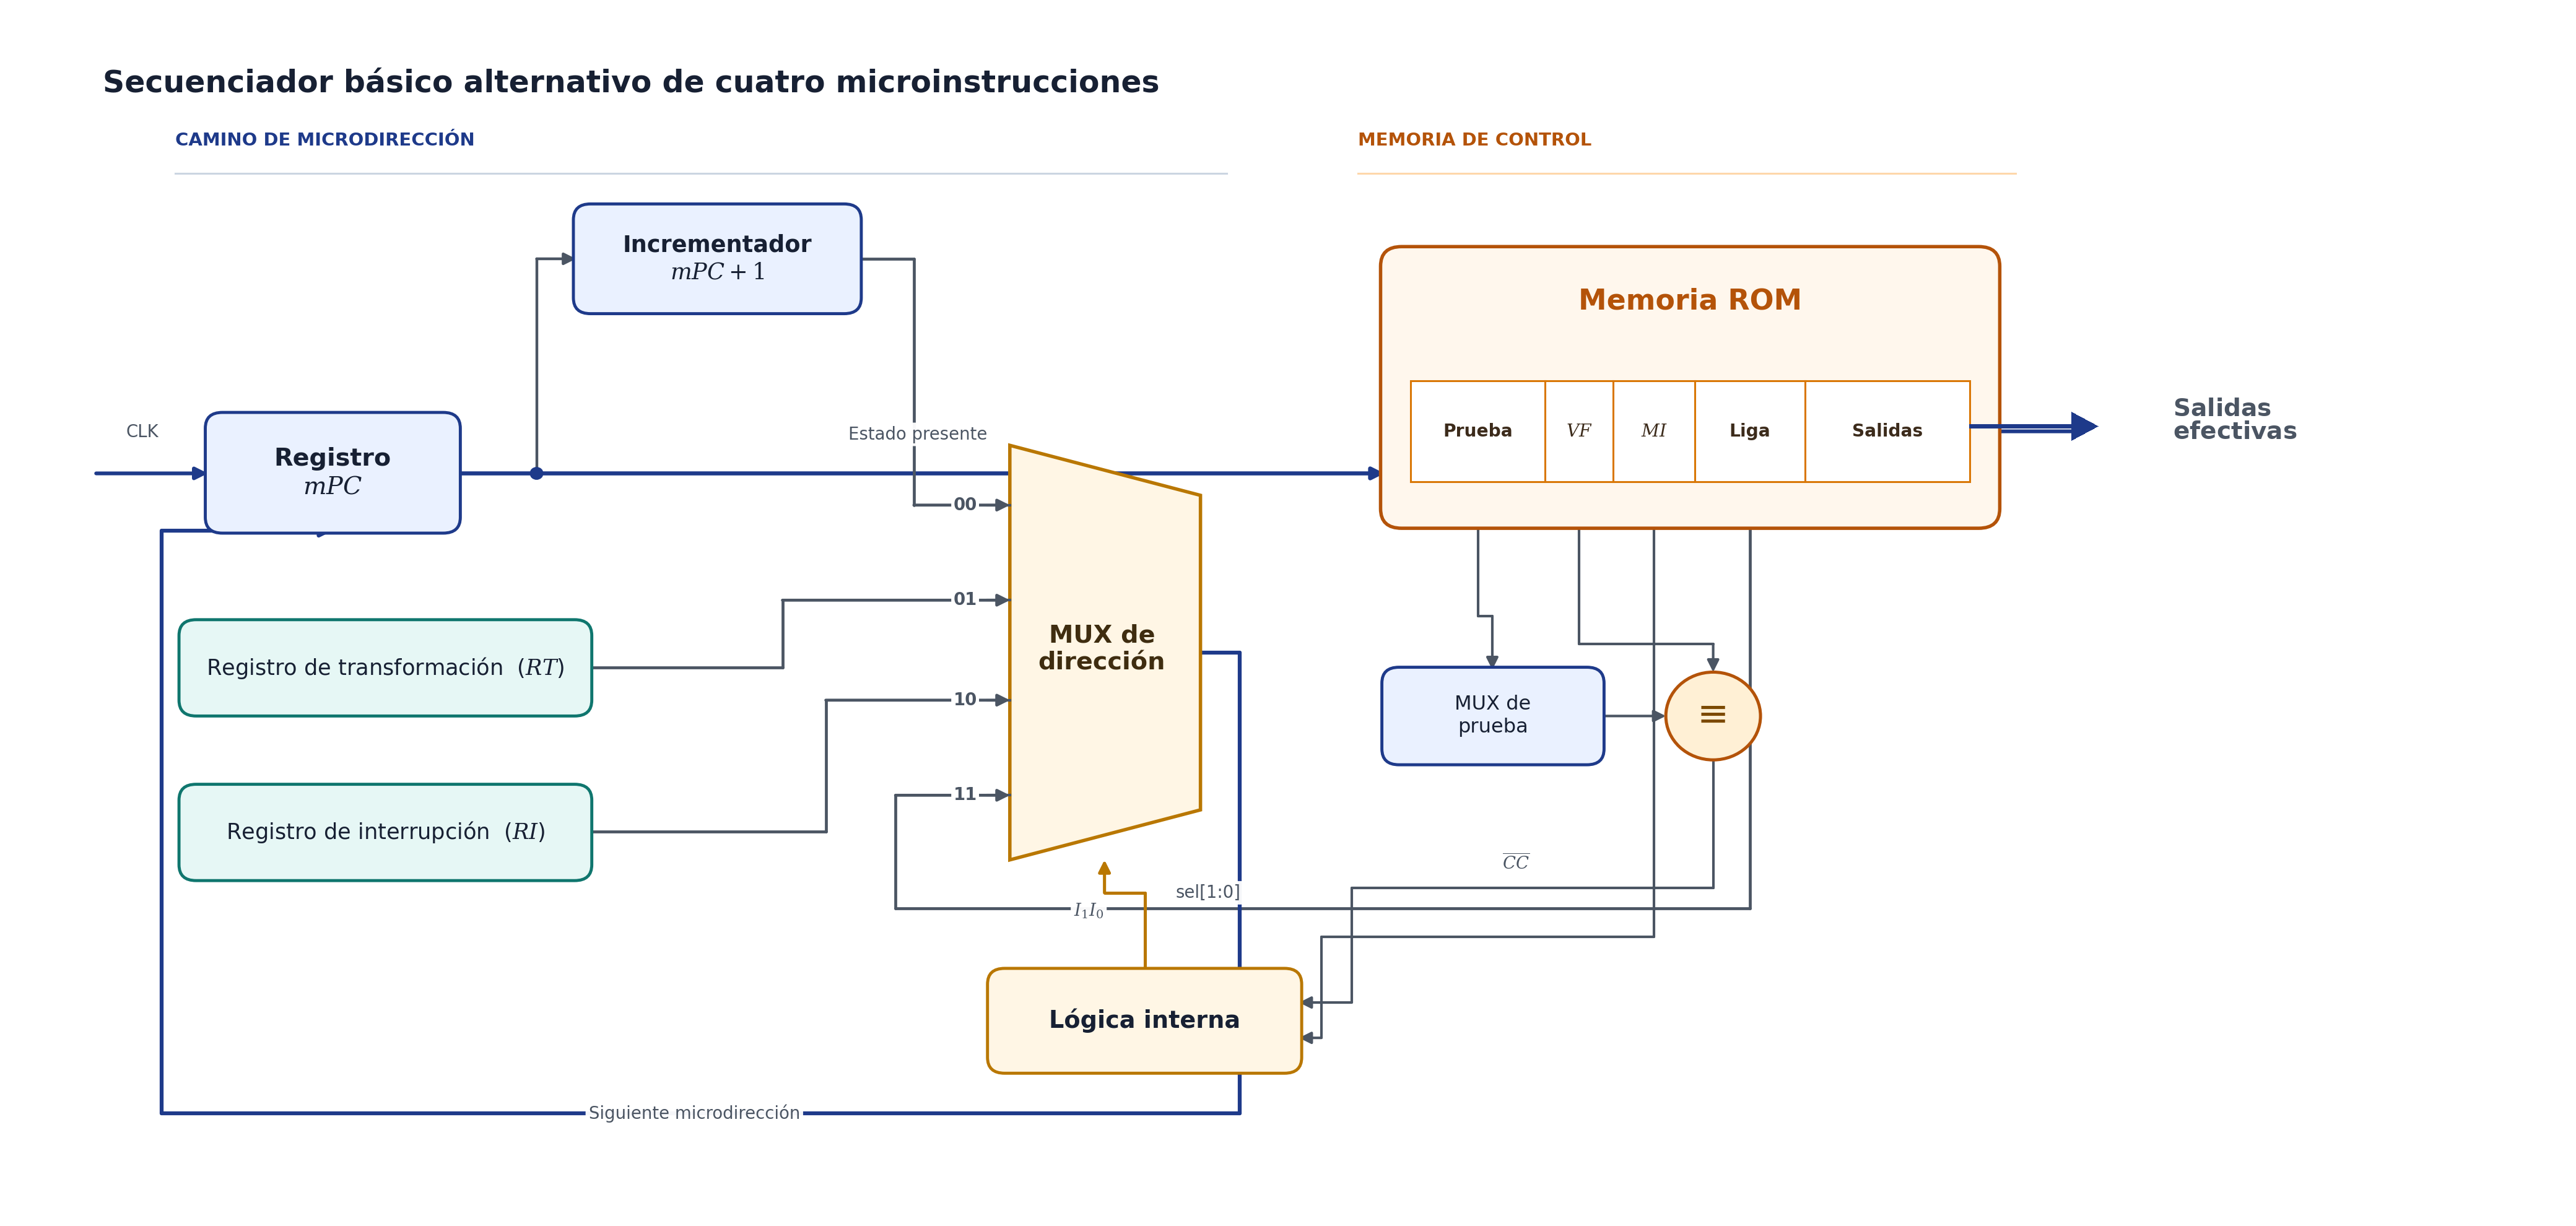
\includegraphics[width=0.98\linewidth]{secuenciador_basico_4mi.png}
\iffalse % Diagrama TikZ anterior; se conserva fuera de compilación.
\resizebox{0.95\linewidth}{!}{%
\begin{tikzpicture}[
  font=\small,
  >=Stealth,
  flow/.style={->, line width=0.85pt, draw=gray!75!black, rounded corners=4pt, line cap=round},
  flowmain/.style={->, line width=1.15pt, draw=blue!70!black, rounded corners=4pt, line cap=round},
  % Estilos de bloques temáticos
  block/.style={
    draw=blue!60!black, fill=blue!8, text=black,
    rounded corners=3pt, line width=0.85pt, align=center,
    inner sep=5pt
  },
  reg/.style={
    draw=teal!60!black, fill=teal!8, text=black,
    rounded corners=3pt, line width=0.85pt, align=center,
    inner sep=5pt, minimum height=0.85cm
  },
  logic/.style={
    draw=amber!70!black, fill=orange!8, text=black,
    rounded corners=3pt, line width=0.85pt, align=center,
    inner sep=5pt
  },
  rombox/.style={
    draw=orange!60!black, fill=orange!5,
    rounded corners=4pt, line width=0.95pt
  },
  labelbox/.style={
    font=\footnotesize, fill=white, inner sep=1.5pt, text=gray!80!black
  },
  portlabel/.style={
    font=\bfseries\scriptsize, fill=white, inner sep=1.5pt, text=gray!90!black
  }
]

  % Bloques que generan y seleccionan la siguiente microdirección
  \node[block, minimum width=2.15cm, minimum height=1.0cm] (mpc) at (-5.4,1.85) {Registro\\$mPC$};
  \node[block, minimum width=2.20cm, minimum height=0.95cm] (inc) at (-2.55,3.45) {Incrementador\\$mPC+1$};
  \node[reg, minimum width=3.05cm] (rt) at (-5.25,0.20) {Registro de transformación ($RT$)};
  \node[reg, minimum width=3.05cm] (ri) at (-5.25,-1.45) {Registro de interrupción ($RI$)};

  % Forma de multiplexor con las cuatro entradas de dirección
  \path[draw=amber!75!black, fill=orange!9, line width=0.95pt]
    (-1.85,1.35) -- (-1.85,-1.85) -- (0.15,-1.20) -- (0.15,0.70) -- cycle;
  \node[align=center] at (-0.90,-0.25) {MUX de\\dirección};
  \coordinate (mux_in00) at (-1.85,0.95);
  \coordinate (mux_in01) at (-1.85,0.28);
  \coordinate (mux_in10) at (-1.85,-0.40);
  \coordinate (mux_in11) at (-1.85,-1.07);
  \coordinate (muxout) at (0.15,-0.25);
  \node[portlabel, anchor=east] at (-1.98,0.95) {00};
  \node[portlabel, anchor=east] at (-1.98,0.28) {01};
  \node[portlabel, anchor=east] at (-1.98,-0.40) {10};
  \node[portlabel, anchor=east] at (-1.98,-1.07) {11};

  % Bloques de prueba y control
  \node[block, minimum width=1.85cm, minimum height=0.85cm] (pmux) at (2.20,-0.72) {MUX de prueba};
  \node[draw=orange!75!black, fill=orange!10, circle, minimum size=0.82cm, line width=0.9pt] (comp) at (4.00,-0.72) {$\equiv$};
  \node[logic, minimum width=2.30cm, minimum height=1.0cm] (logica) at (-0.82,-3.25) {Lógica interna};

  % =========================================================================
  % 2. MEMORIA ROM
  % =========================================================================
  % Caja contenedora
  \draw[rombox] (1.45, 0.80) rectangle (6.35, 3.25);
  \node[font=\bfseries\large, text=orange!55!black] at (3.90, 2.90) {Memoria ROM};

  % Campos de la microinstrucción
  \draw[fill=white, draw=orange!45!black, line width=0.65pt] (1.70, 1.15) rectangle (6.10, 2.35);
  \draw[draw=orange!40!black, line width=0.6pt] 
    (2.55, 1.15) -- (2.55, 2.35)
    (3.10, 1.15) -- (3.10, 2.35)
    (3.75, 1.15) -- (3.75, 2.35)
    (4.65, 1.15) -- (4.65, 2.35);

  \node[font=\scriptsize\bfseries] (f_prueba) at (2.12, 1.75) {Prueba};
  \node[font=\scriptsize\bfseries] (f_vf)     at (2.83, 1.75) {$VF$};
  \node[font=\scriptsize\bfseries] (f_mi)     at (3.42, 1.75) {$MI$};
  \node[font=\scriptsize\bfseries] (f_liga)   at (4.20, 1.75) {Liga};
  \node[font=\scriptsize\bfseries] (f_sal)    at (5.37, 1.75) {Salidas};

  % Reloj, dirección presente e incremento
  \draw[flowmain] (-7.05,1.85) -- (mpc.west) node[pos=0.28, above, labelbox] {\textbf{CLK}};
  \draw[flowmain] (mpc.east) -- (1.45,1.85) -- (1.45,2.00)
    node[pos=0.58, above, labelbox] {\textbf{Estado presente}};
  \fill[blue!70!black] (-3.55,1.85) circle (1.3pt);
  \draw[flow] (-3.55,1.85) |- (inc.west);

  % Fuentes de la siguiente dirección
  \draw[flow] (inc.east) -| (mux_in00);
  \draw[flow] (rt.east) -- (mux_in01);
  \draw[flow] (ri.east) -- (-2.55,-1.45) |- (mux_in10);
  \draw[flow] (f_liga.south) -- (4.20,-2.12) -- (-2.25,-2.12) |- (mux_in11);

  % Realimentación de la siguiente microdirección al mPC
  \draw[flowmain] (muxout) -- (0.62,-0.25) |- (-6.75,-4.15) |- (mpc.south);
  \node[labelbox] at (-3.25,-4.15) {Siguiente microdirección};

  % Prueba, comparación y señales de control
  \draw[flow] (f_prueba.south) -- (2.12,-0.15) -| (pmux.north);
  \draw[flow] (pmux.east) -- (comp.west);
  \draw[flow] (f_vf.south) -- (2.83,-0.12) -| (comp.north);
  \draw[flow] (comp.south) -- (4.00,-2.45) -- (0.55,-2.45) |- ([yshift=3pt]logica.east)
    node[pos=0.32, above, labelbox] {$\overline{CC}$};
  \draw[flow] (f_mi.south) -- (3.42,-2.82) -- (0.55,-2.82) |- ([yshift=-3pt]logica.east)
    node[pos=0.28, above, labelbox] {$I_1I_0$};
  \draw[flow] (logica.north) -- (-0.82,-1.95)
    node[midway, right=2pt, portlabel] {sel[1:0]};

  % Salidas efectivas de la microinstrucción
  \draw[flowmain] (6.10,1.75) -- (7.20,1.75);
  \node[align=left, font=\bfseries\small, text=gray!85!black, anchor=west] at (7.25,1.75) {Salidas\\efectivas};

\end{tikzpicture}%
}
\fi
\caption{Diagrama del secuenciador básico alternativo de cuatro microinstrucciones.}
\label{fig:secuenciador-general}
\end{figure}


Las cuatro opciones se definen con los bits $I_1I_0$. El paso continuo selecciona el valor $mPC+1$. El salto condicional selecciona la liga solamente cuando $CC=0$. El salto de transformación usa el registro $RT$ sin depender de $CC$. Finalmente, la microinstrucción de interrupción selecciona el registro $RI$ cuando $CC=0$; si la condición no solicita la interrupción, el contador continúa normalmente.

\begin{table}[H]
\centering
\small
\caption{Tabla de operación del secuenciador básico alternativo.}
\label{tab:microinstrucciones}
\begin{tabular}{c c c c l}
\toprule
$I_1$ & $I_0$ & $CC$ & \texttt{sel} & Operación realizada \\
\midrule
0 & 0 & $X$ & 00 & Paso continuo: $mPC \leftarrow mPC+1$. \\
0 & 1 & 0 & 11 & Salto condicional: $mPC \leftarrow \text{Liga}$. \\
0 & 1 & 1 & 00 & No se cumple el salto: $mPC \leftarrow mPC+1$. \\
1 & 0 & $X$ & 01 & Salto de transformación: $mPC \leftarrow RT$. \\
1 & 1 & 0 & 10 & Salto de interrupción: $mPC \leftarrow RI$. \\
1 & 1 & 1 & 00 & No hay interrupción: $mPC \leftarrow mPC+1$. \\
\bottomrule
\end{tabular}
\end{table}

Para la demostración se usaron las direcciones fijas de la Tabla~\ref{tab:direcciones}. Estos valores permiten distinguir claramente cada fuente cuando se observa la salida del contador de microprograma. El incremento se obtiene de manera combinacional a partir de la dirección presente.

\begin{table}[H]
\centering
\caption{Fuentes de dirección utilizadas en la implementación.}
\label{tab:direcciones}
\begin{tabular}{l c c}
\toprule
Fuente & Dirección de prueba & Selección del multiplexor \\
\midrule
Paso continuo & $mPC+1$ & 00 \\
Registro de liga & \texttt{1000} & 11 \\
Registro de transformación ($RT$) & \texttt{1010} & 01 \\
Registro de interrupción ($RI$) & \texttt{1100} & 10 \\
\bottomrule
\end{tabular}
\end{table}

\subsection{Arquitectura implementada}

El registro $mPC$ conserva la microdirección presente y se actualiza únicamente en el flanco ascendente del reloj. Su salida se realimenta al incrementador, el cual genera $mPC+1$. El multiplexor recibe cuatro posibles direcciones: la consecutiva, la liga, $RT$ y $RI$. La lógica interna entrega la señal \texttt{sel[1..0]} que determina cuál de ellas llegará al registro $mPC$ en el siguiente pulso.

La Figura~\ref{fig:interconexion} muestra la conexión final de los módulos. La señal de reloj se acondiciona mediante el bloque \texttt{clk\_buttom}, con el fin de avanzar una microinstrucción a la vez desde el botón de la tarjeta. Las entradas $I_0$, $I_1$ y $CC$ alimentan la lógica interna; la salida \texttt{edo\_pr[3..0]} permite observar la microdirección presente.

\begin{figure}[H]
\centering
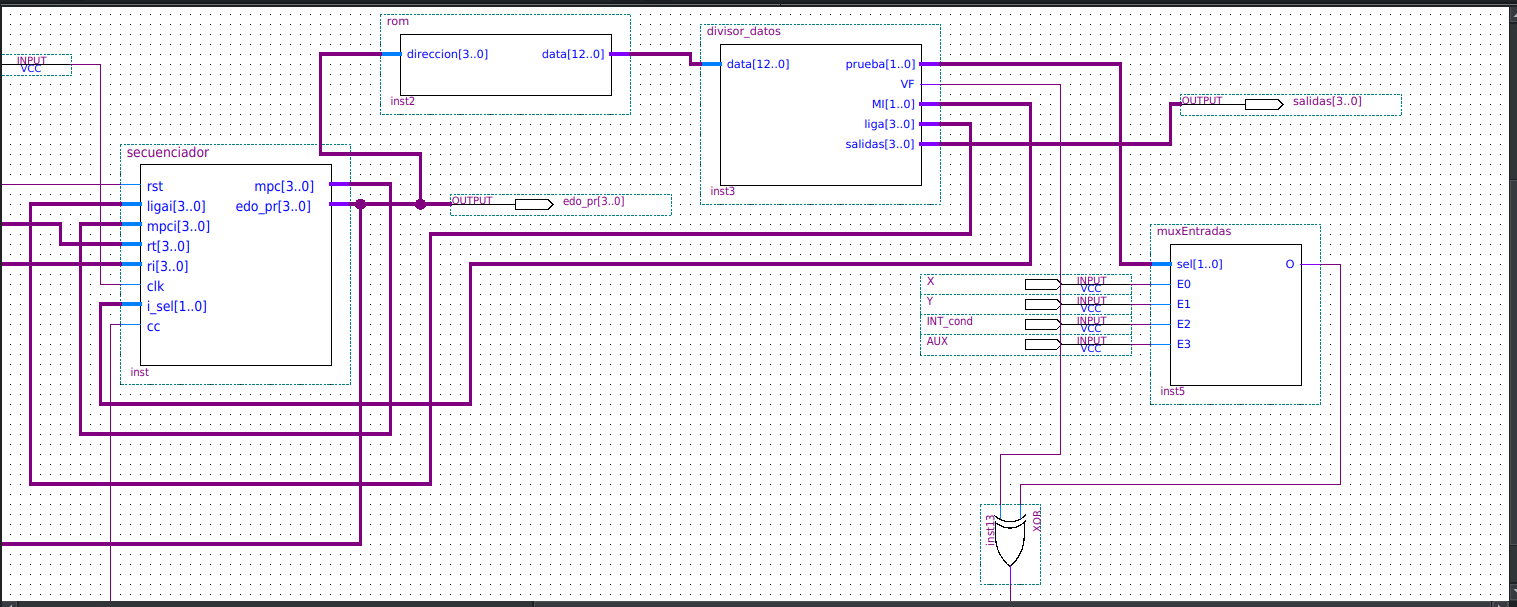
\includegraphics[width=\linewidth]{diagramas_bloques_2.png}
\caption{Interconexión final del multiplexor, los registros, la lógica interna y el contador de microprograma.}
\label{fig:interconexion}
\end{figure}

En la Figura~\ref{fig:contador-mpc} se observa con mayor detalle la realimentación entre el registro $mPC$ y el incrementador. El valor incrementado entra a la primera opción del multiplexor y constituye el recorrido natural del microprograma cuando se selecciona el paso continuo.

\begin{figure}[H]
\centering
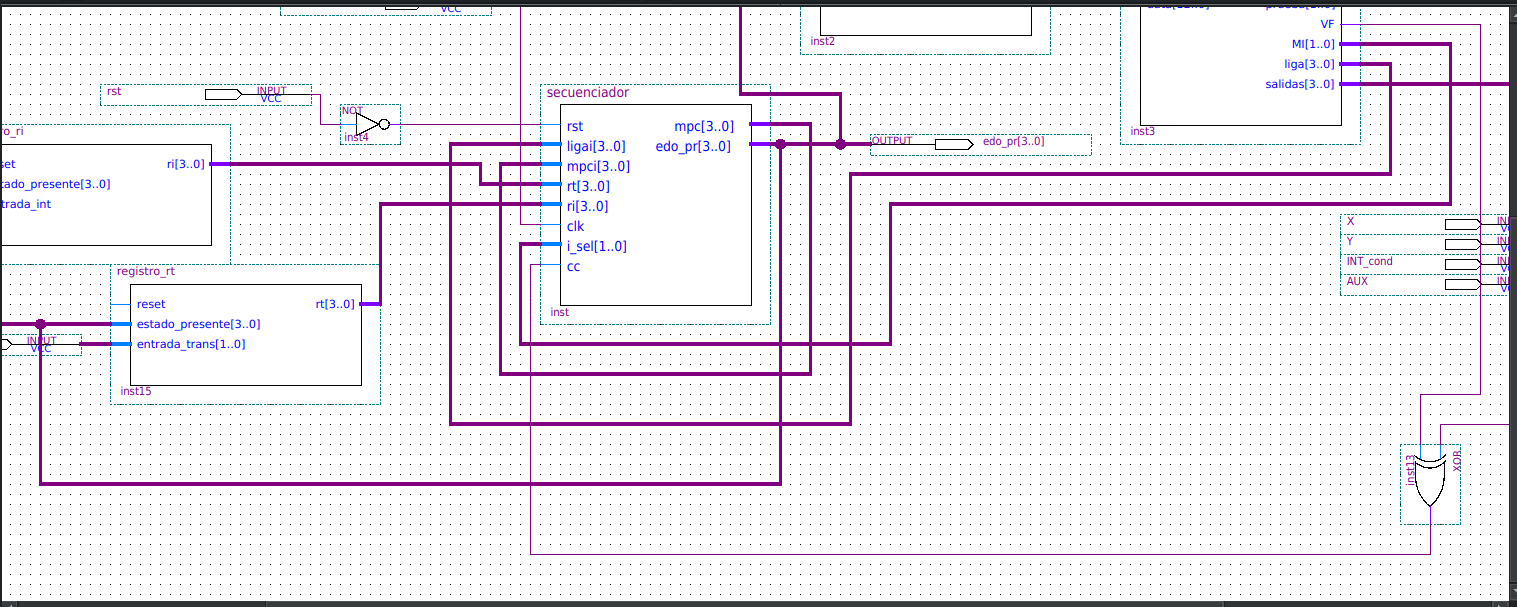
\includegraphics[width=0.92\linewidth]{diagramas_bloques_3.png}
\caption{Camino de realimentación para el paso continuo $mPC+1$.}
\label{fig:contador-mpc}
\end{figure}

\subsection{Módulos implementados en VHDL}

\paragraph{Contador de microprograma e incrementador.} El módulo \texttt{registro\_mpc} almacena la dirección que entrega el multiplexor. El reinicio es asíncrono y activo en bajo, por lo que \texttt{reset='0'} fuerza la dirección \texttt{0000}. El incrementador calcula de forma combinacional la dirección consecutiva de cuatro bits.

\lstinputlisting[style=estiloVHDL,caption={Registro del contador de microprograma.},label={lst:registro-mpc}]{code/registro_mpc.vhd}

\lstinputlisting[style=estiloVHDL,caption={Incrementador que genera $mPC+1$.},label={lst:incrementador}]{code/incrementador.vhd}

\paragraph{Multiplexor y lógica interna.} El multiplexor \texttt{mux} concentra las cuatro fuentes de dirección. La lógica combinacional convierte los bits $I_1I_0$ y la condición \texttt{cc} en el selector de dos bits, de acuerdo con la Tabla~\ref{tab:microinstrucciones}.

\lstinputlisting[style=estiloVHDL,caption={Multiplexor de cuatro fuentes para la siguiente microdirección.},label={lst:mux}]{code/mux.vhd}

\lstinputlisting[style=estiloVHDL,caption={Lógica interna que implementa los cuatro tipos de microinstrucción.},label={lst:logica}]{code/logica.vhd}

\paragraph{Registros de dirección.} Los registros de liga, transformación e interrupción entregan valores constantes después de liberar el reinicio: \texttt{1000}, \texttt{1010} y \texttt{1100}, respectivamente. Su función en la práctica es representar las direcciones que seleccionaría el secuenciador.

\lstinputlisting[style=estiloVHDL,caption={Registro que entrega la dirección de liga.},label={lst:liga}]{code/registro_liga.vhd}

\lstinputlisting[style=estiloVHDL,caption={Registro de dirección de transformación.},label={lst:rt}]{code/registro_rt.vhd}

\lstinputlisting[style=estiloVHDL,caption={Registro de dirección de interrupción.},label={lst:ri}]{code/registro_ri.vhd}

\paragraph{Reloj por botón.} El bloque \texttt{clk\_buttom} genera un pulso lento y controlable a partir del reloj de la FPGA y del botón. De esta forma fue posible comprobar cada cambio de dirección en los LEDs sin que el secuenciador avanzara demasiado rápido.

\lstinputlisting[style=estiloVHDL,caption={Generación de un pulso de reloj controlado por botón.},label={lst:clk-button}]{code/clk_buttom.vhd}

\section{Simulación}

La simulación se realizó con una señal de reloj periódica, reinicio activo en bajo y diferentes combinaciones de $I_1$, $I_0$ y $CC$. La señal \texttt{edo\_pr} muestra el contenido del contador de microprograma. Debido a que $mPC$ es un registro, cada dirección se actualiza en el flanco ascendente del reloj y permanece estable entre flancos.

En la Figura~\ref{fig:simulacion-1} se observan los cuatro valores importantes del diseño. Además de los avances consecutivos como \texttt{1000}$\rightarrow$\texttt{1001}$\rightarrow$\texttt{1010}, aparecen \texttt{1000} por la liga, \texttt{1010} por el registro de transformación y \texttt{1100} por el registro de interrupción. Esto permite reconocer la fuente seleccionada a partir de la salida del contador.

\begin{figure}[H]
\centering
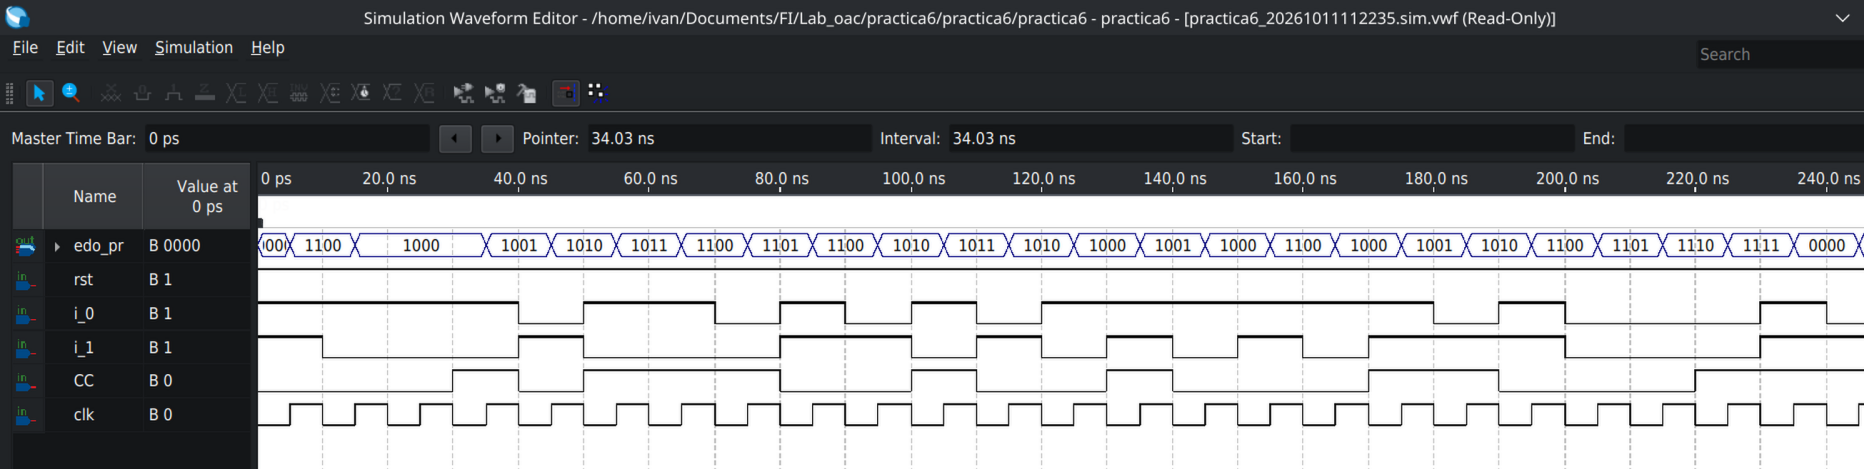
\includegraphics[width=\linewidth]{simulacion_1.png}
\caption{Primera parte de la simulación funcional del secuenciador.}
\label{fig:simulacion-1}
\end{figure}

La Figura~\ref{fig:simulacion-2} verifica la respuesta de la lógica interna al cambiar las entradas durante la simulación. Cuando $I_1I_0=01$, el valor de $CC$ decide entre el salto a la liga y el paso continuo. Para $I_1I_0=10$, la salida toma directamente el valor del registro $RT$. Para $I_1I_0=11$, sólo se usa el registro $RI$ cuando $CC=0$.

\begin{figure}[H]
\centering
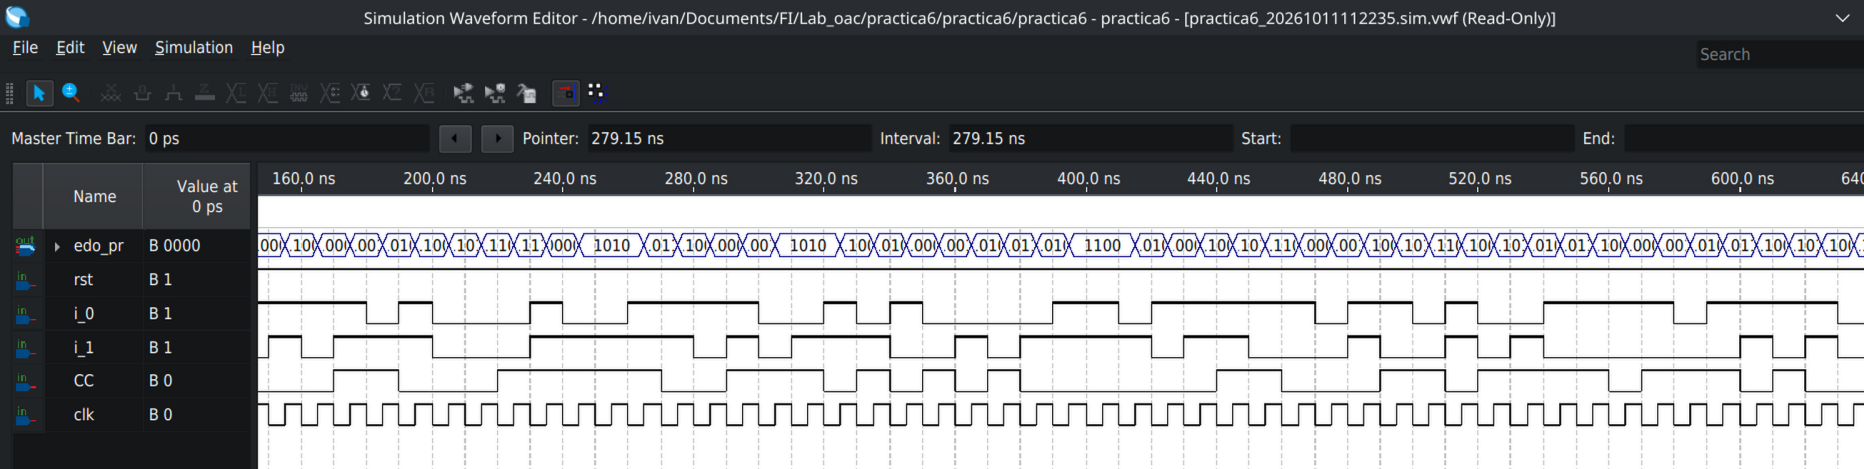
\includegraphics[width=\linewidth]{simulacion_2.png}
\caption{Cambios de microdirección al modificar $I_1$, $I_0$ y $CC$.}
\label{fig:simulacion-2}
\end{figure}

En la parte final, mostrada en la Figura~\ref{fig:simulacion-3}, se repiten los modos de operación con nuevas combinaciones de entrada. La señal \texttt{edo\_pr} no depende directamente de los cambios intermedios de las entradas, sino del valor que la lógica seleccione al siguiente flanco de reloj. Con ello se comprueba la operación síncrona del secuenciador.

\begin{figure}[H]
\centering
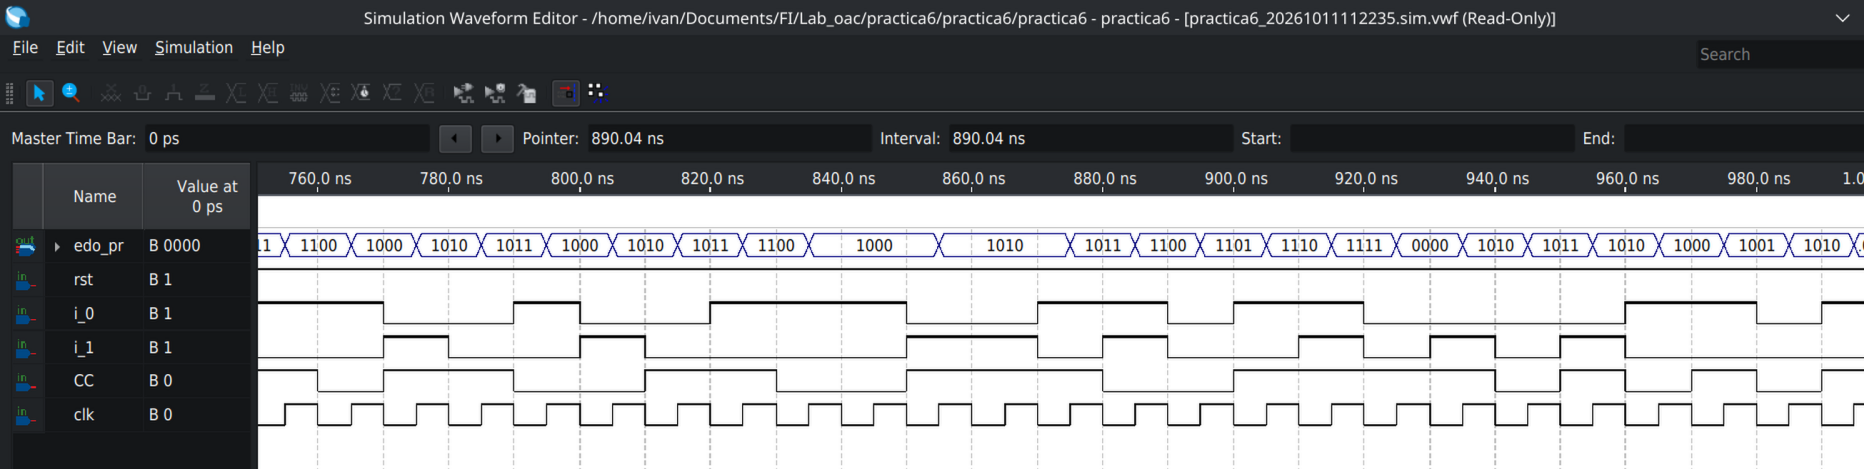
\includegraphics[width=\linewidth]{simulacion_3.png}
\caption{Parte final de la simulación, con recorridos continuos y saltos.}
\label{fig:simulacion-3}
\end{figure}

\section{Resultados en la tarjeta FPGA}

El diseño se implementó en la tarjeta de desarrollo DE10-Lite. Las fotografías muestran distintas combinaciones de $I_1I_0CC$ y los LEDs asociados a la microdirección presente. Cada combinación activa la fuente indicada en la Tabla~\ref{tab:microinstrucciones}, por lo que se pueden distinguir visualmente los modos continuo, condicional, de transformación y de interrupción.

\begin{figure}[H]
\centering
\begin{subfigure}[b]{0.47\linewidth}
  \centering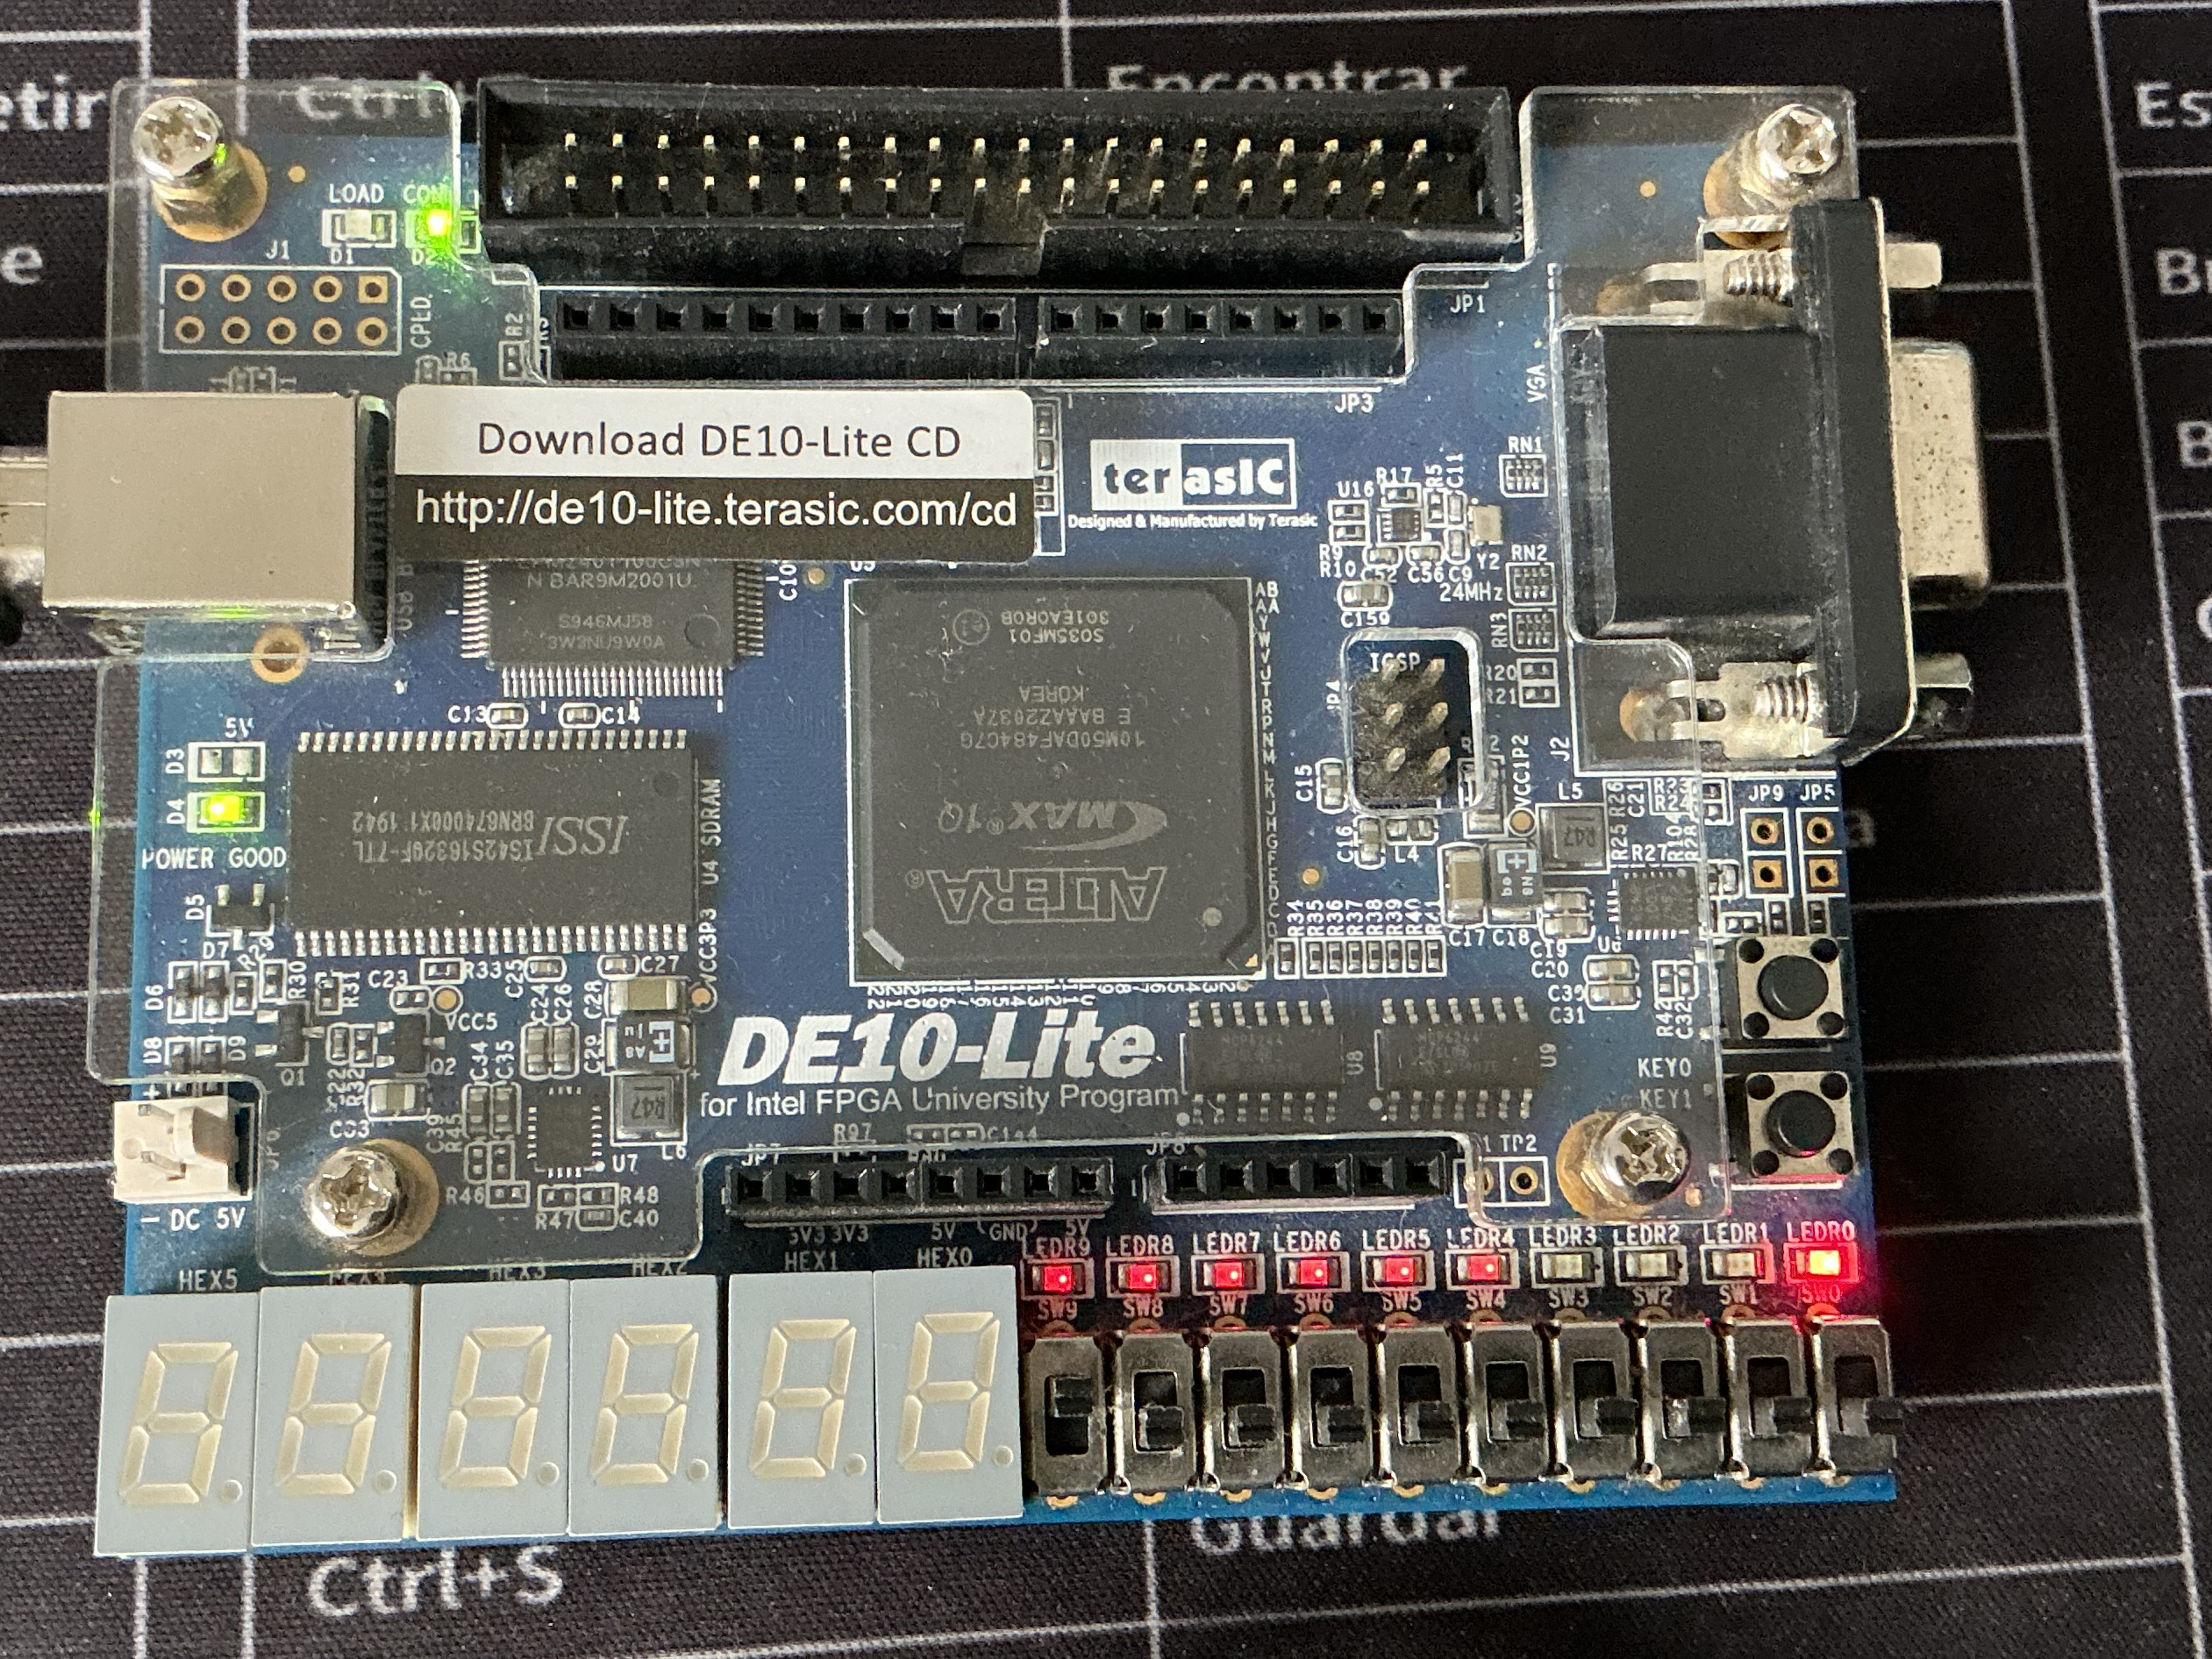
\includegraphics[width=\linewidth]{000_i2i1cc.jpeg}
  \caption{Combinación \texttt{000}: paso continuo.}
\end{subfigure}\hfill
\begin{subfigure}[b]{0.47\linewidth}
  \centering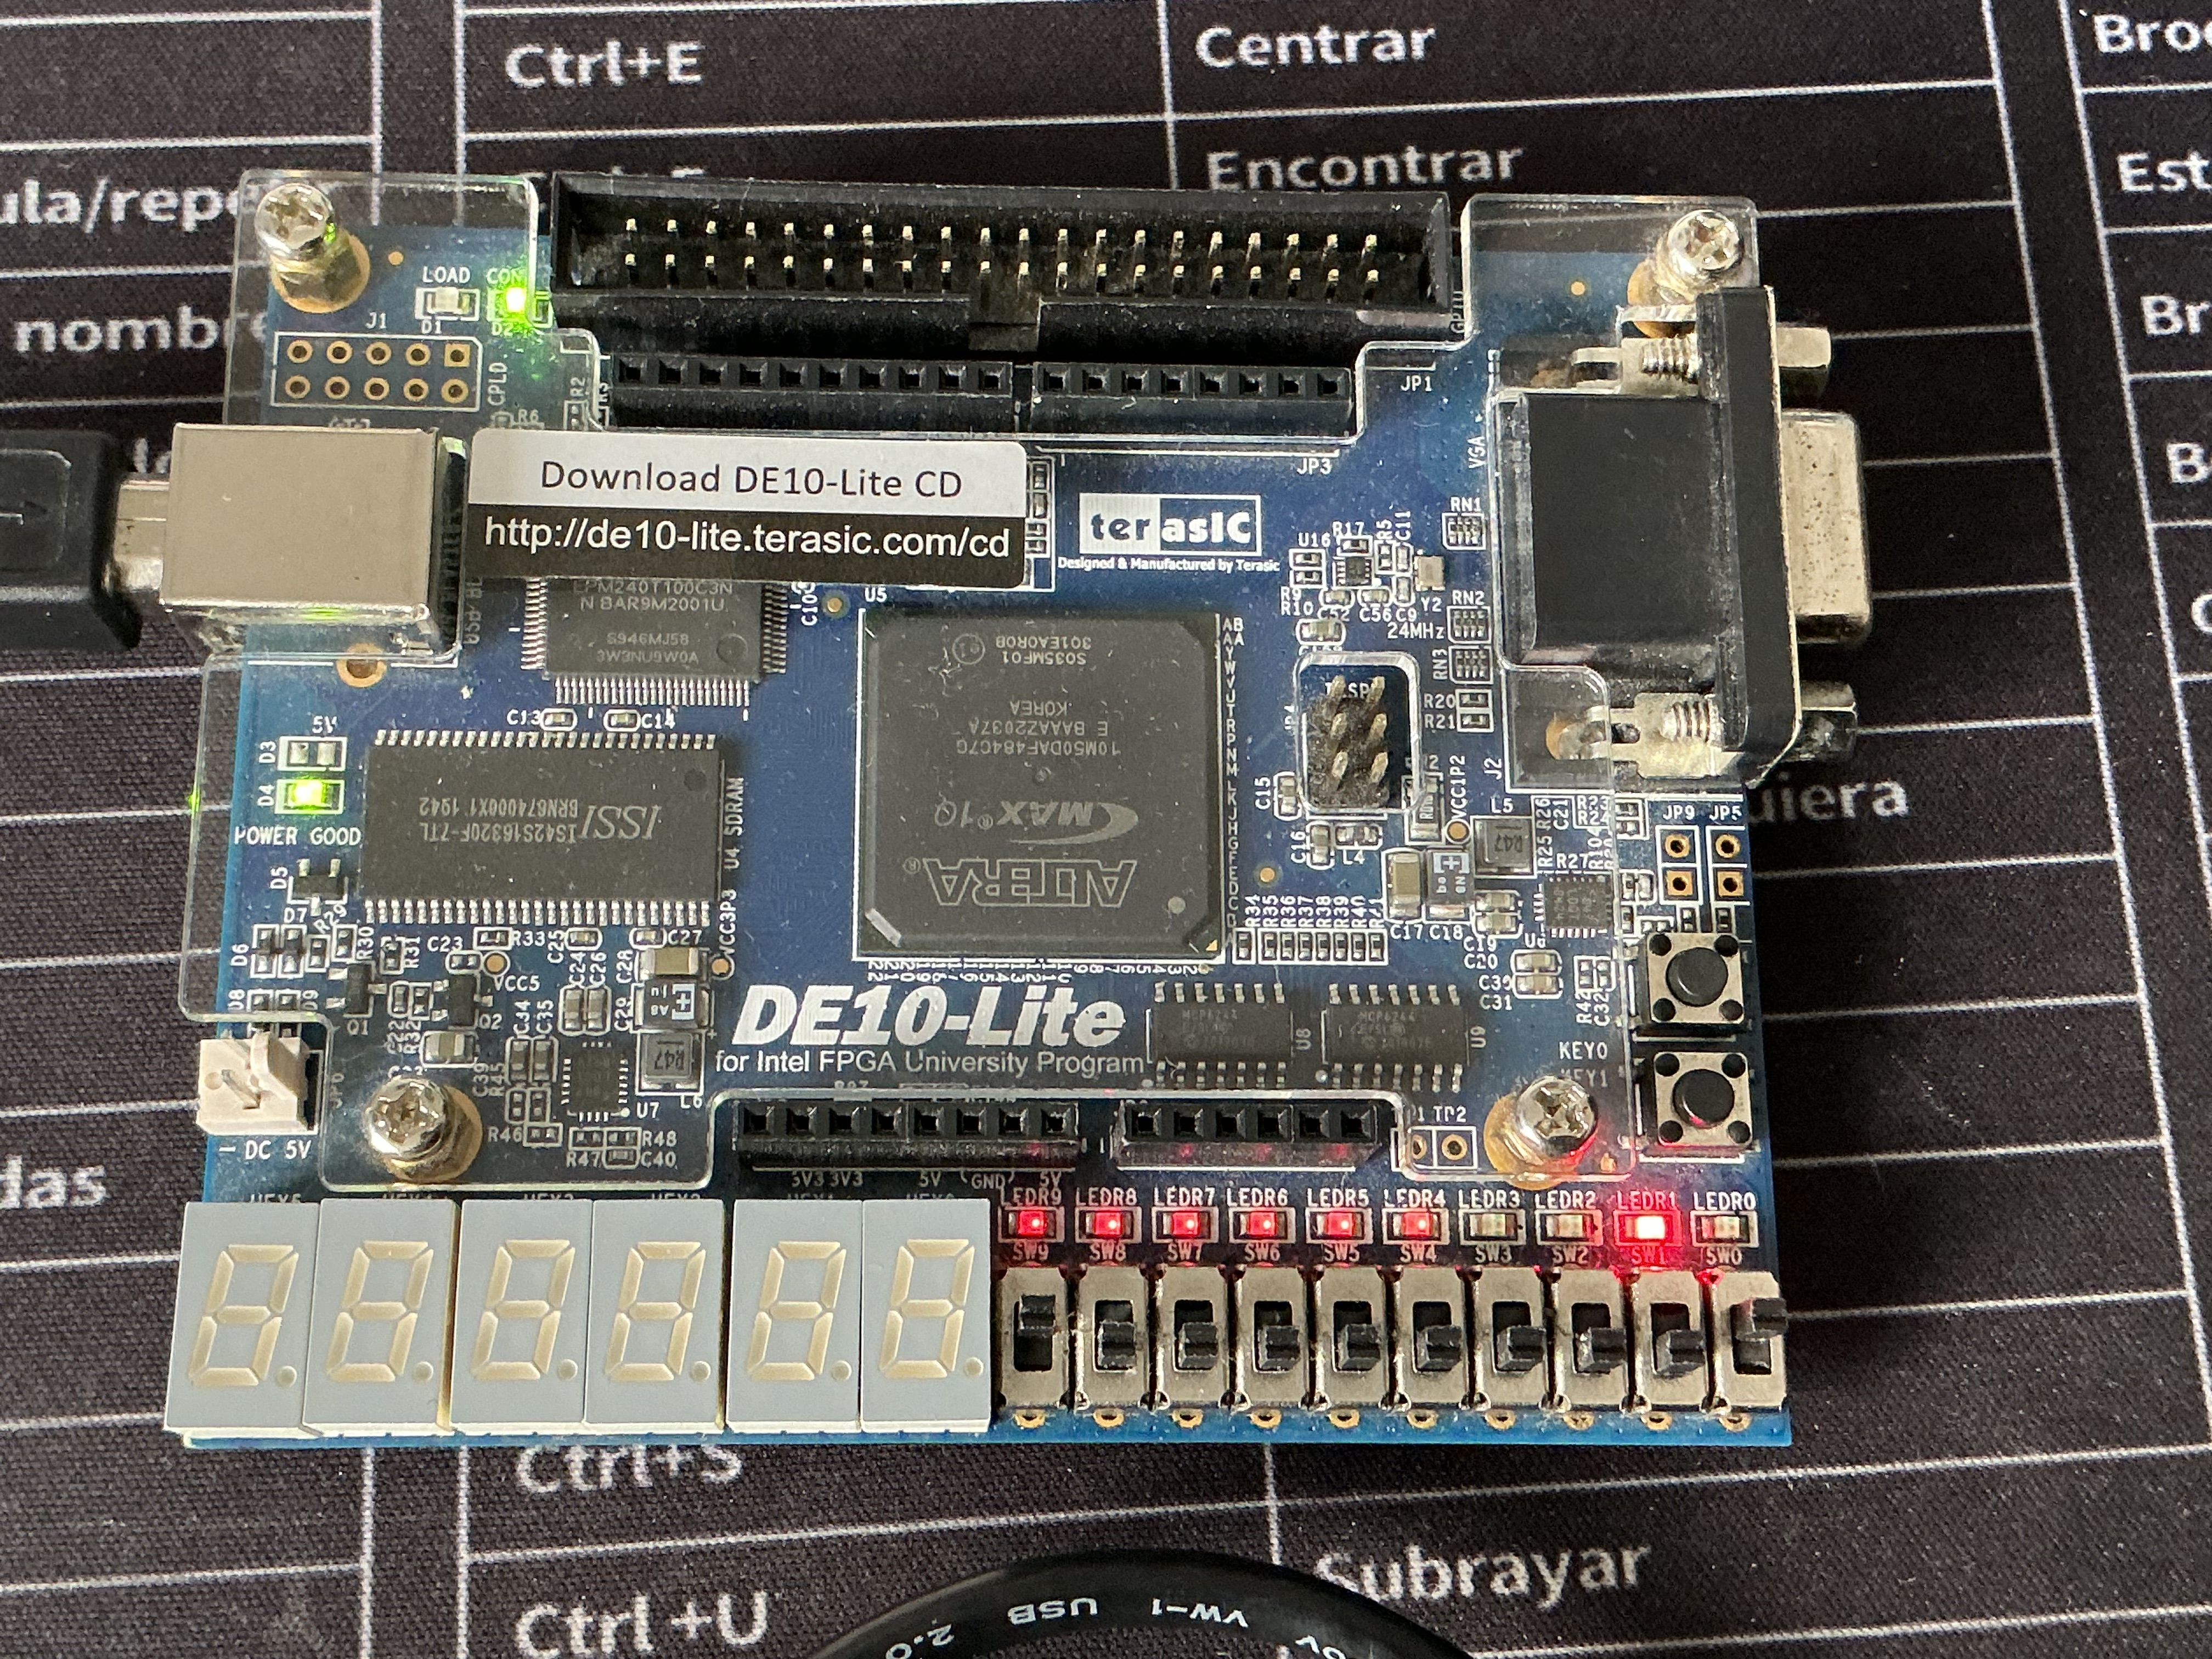
\includegraphics[width=\linewidth]{001.jpeg}
  \caption{Combinación \texttt{001}: paso continuo.}
\end{subfigure}
\caption{Comprobación física del modo $I_1I_0=00$.}
\label{fig:fpga-00}
\end{figure}

\begin{figure}[H]
\centering
\begin{subfigure}[b]{0.47\linewidth}
  \centering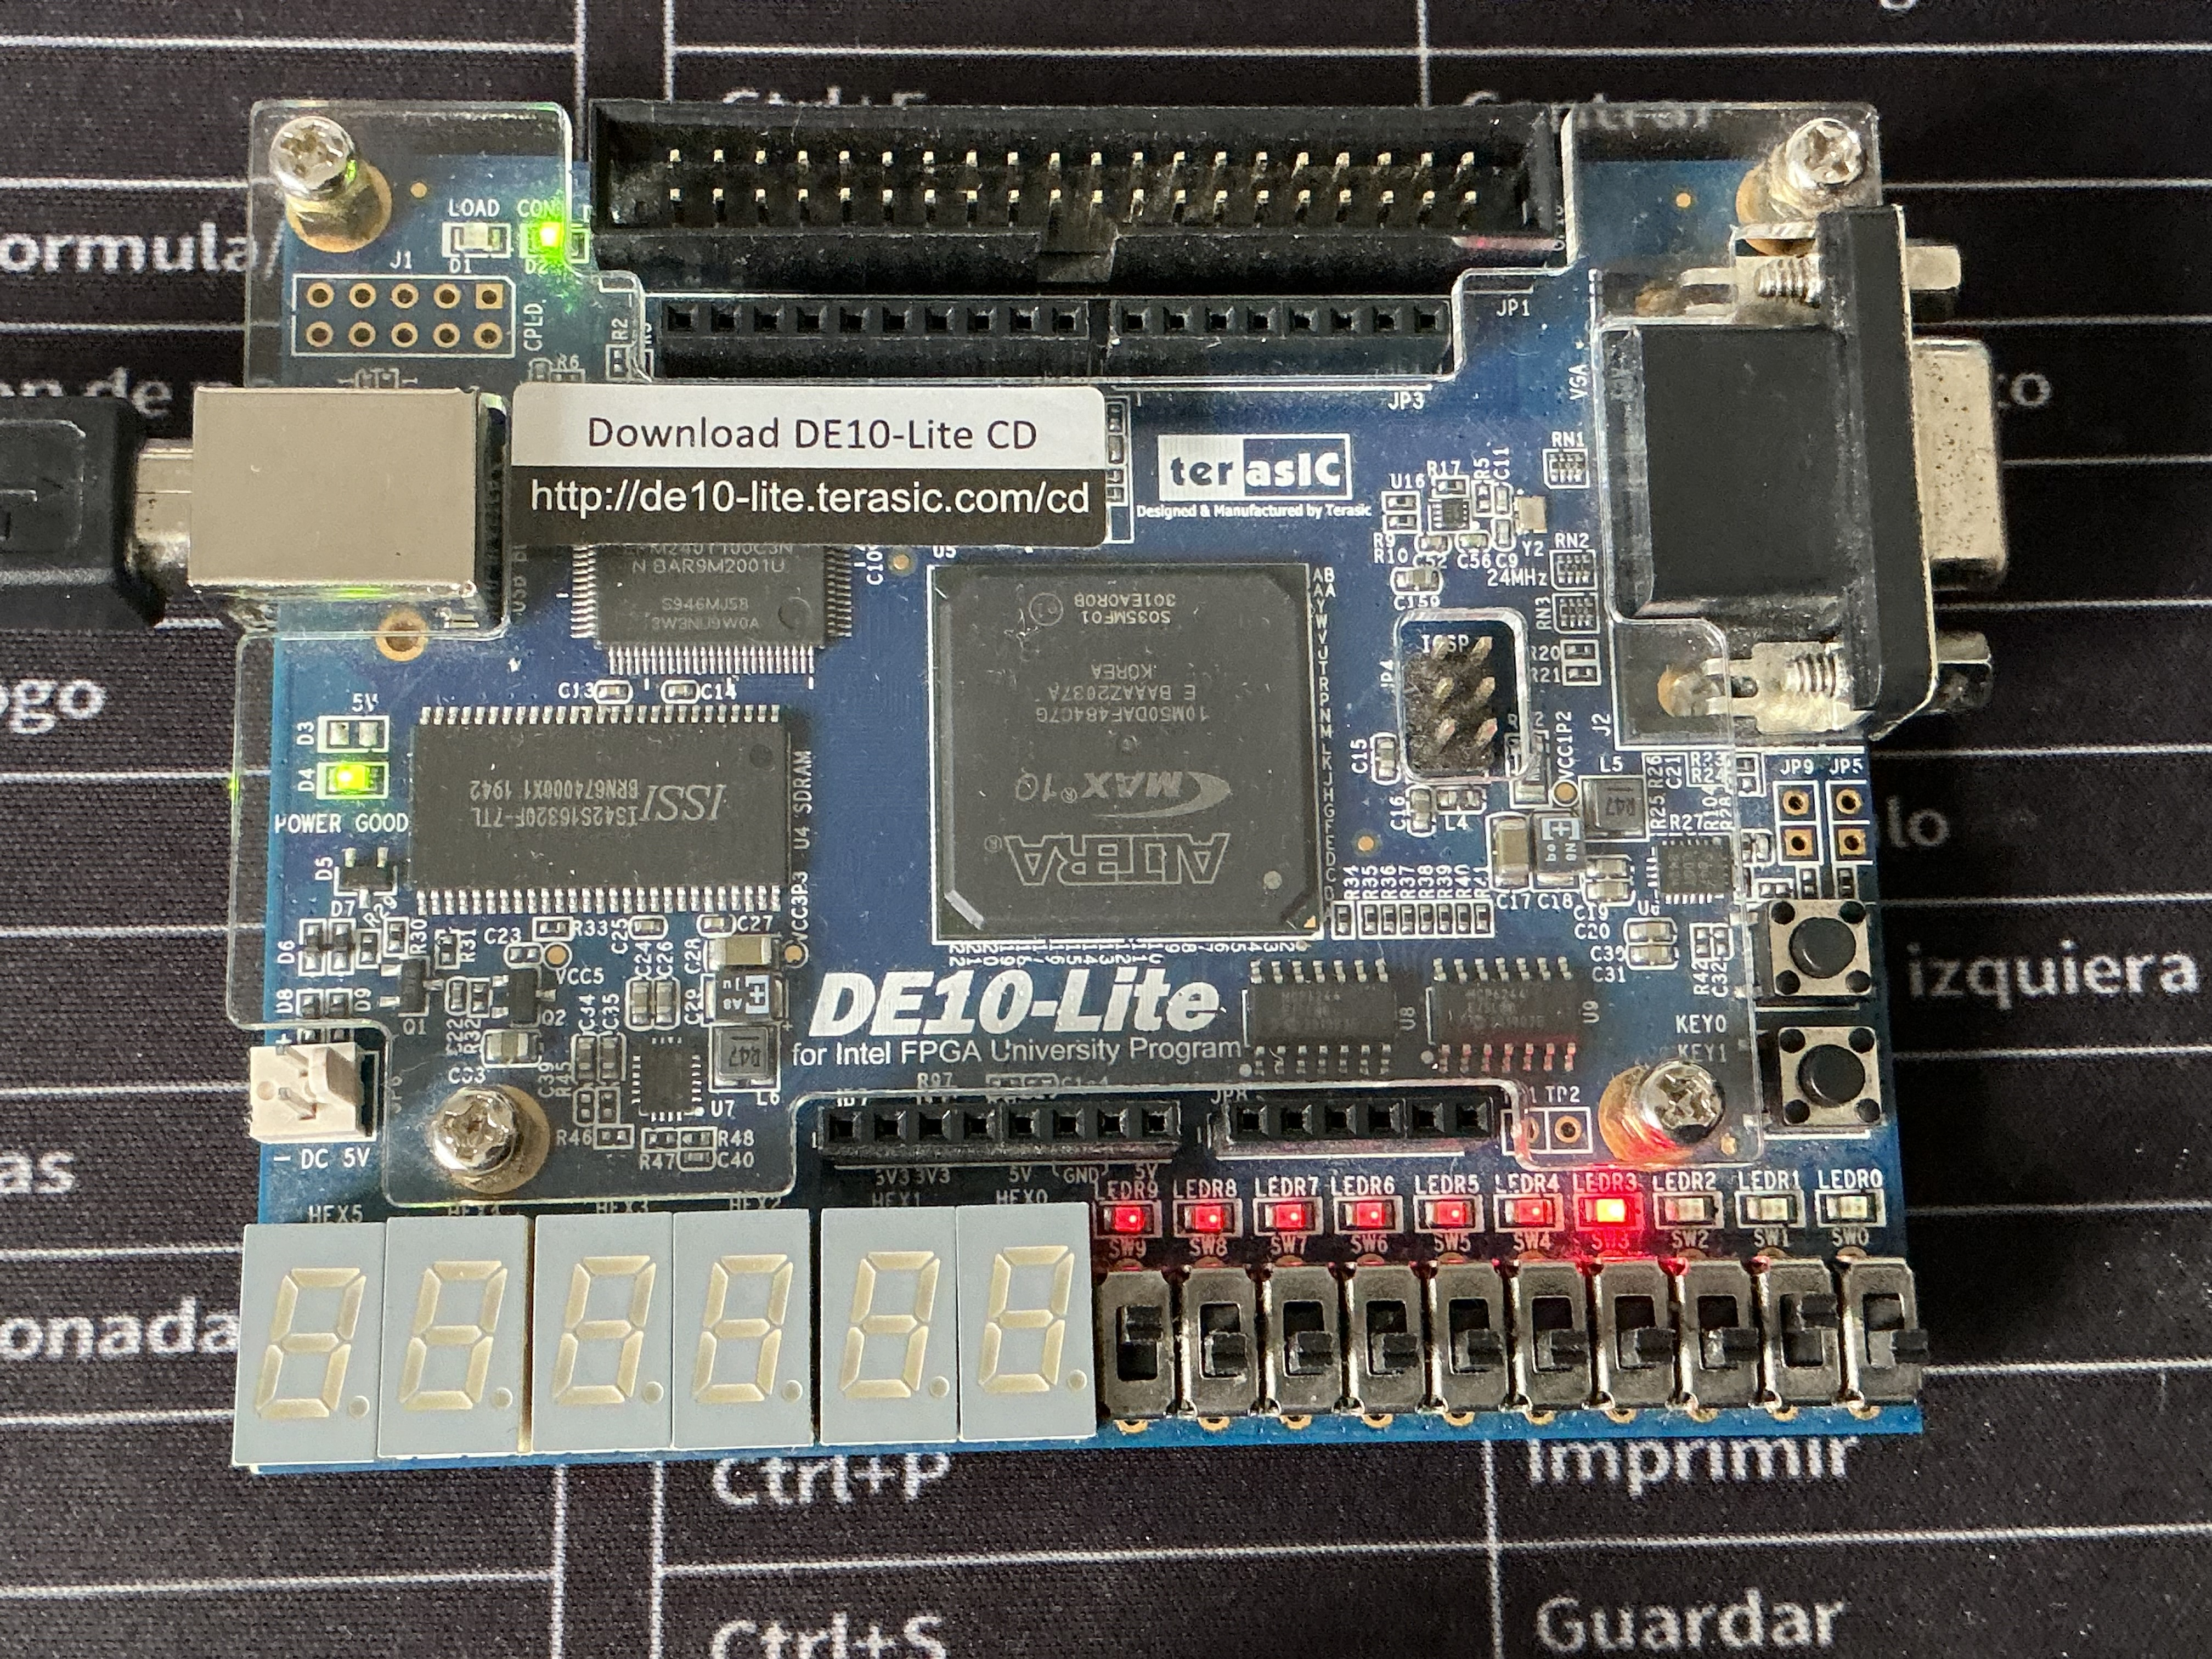
\includegraphics[width=\linewidth]{010.jpeg}
  \caption{\texttt{010}: salto condicional a la liga.}
\end{subfigure}\hfill
\begin{subfigure}[b]{0.47\linewidth}
  \centering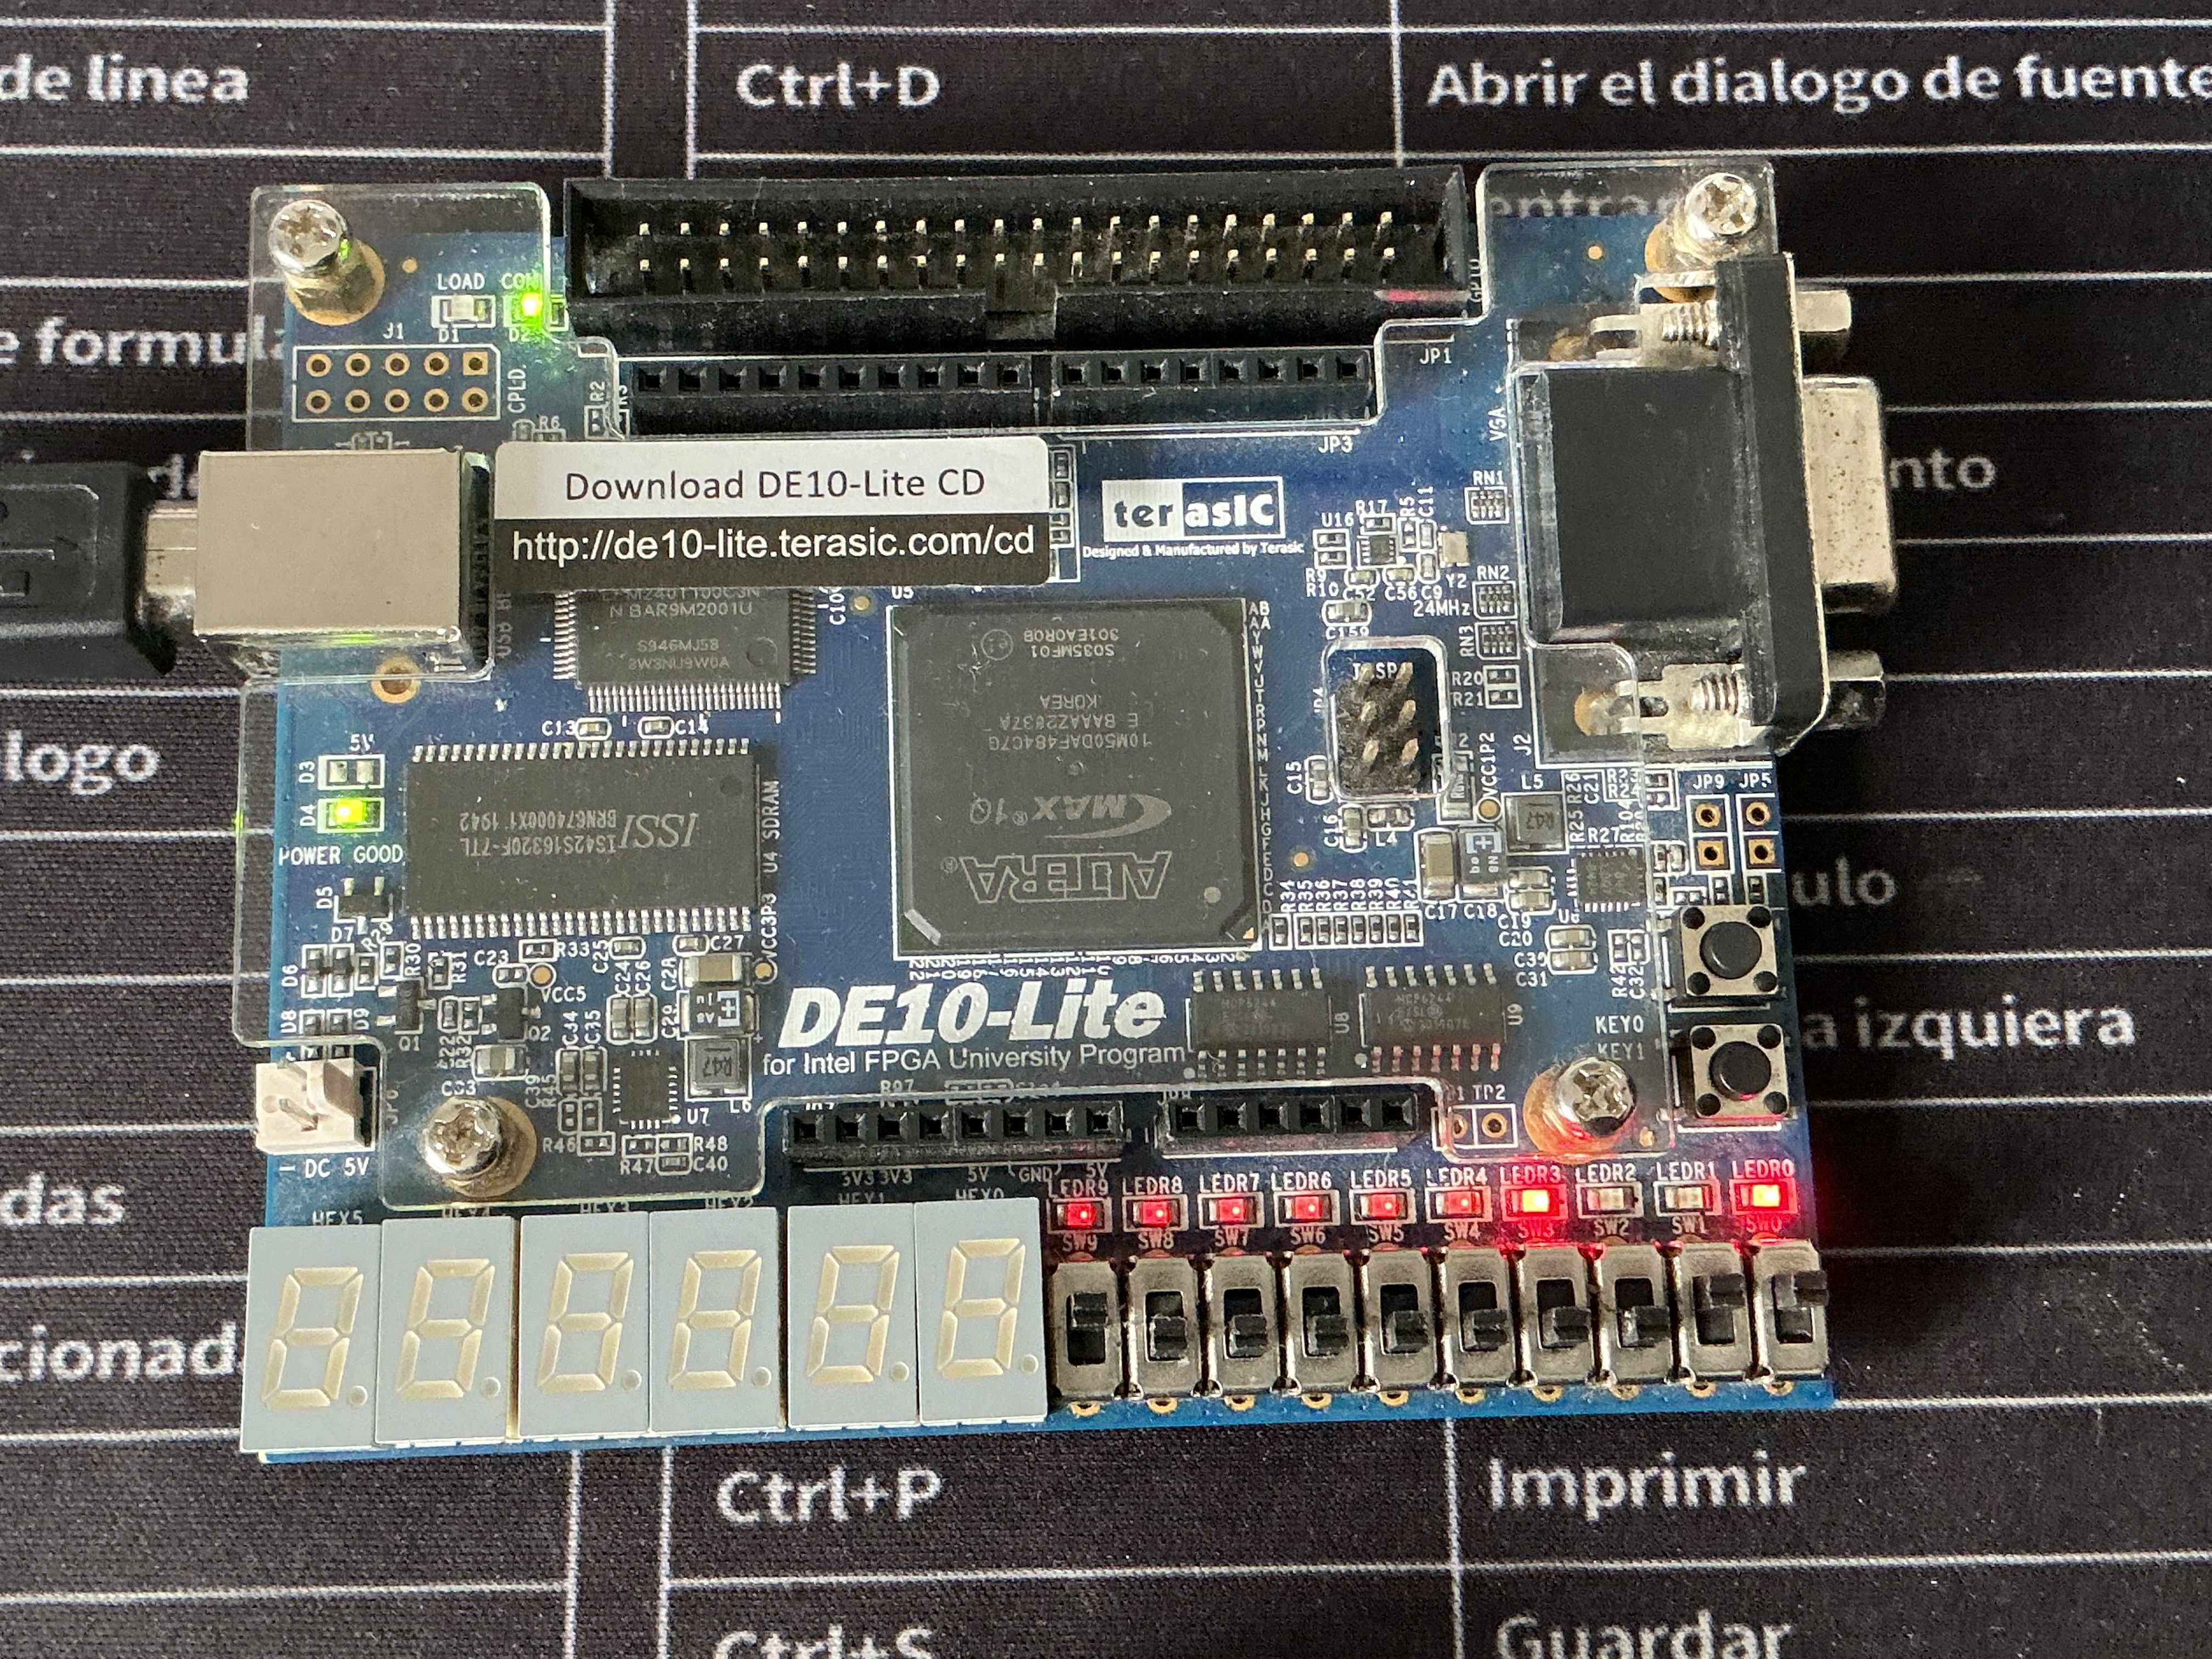
\includegraphics[width=\linewidth]{011.jpeg}
  \caption{\texttt{011}: avance continuo.}
\end{subfigure}
\caption{Comprobación del salto condicionado por $CC$ para $I_1I_0=01$.}
\label{fig:fpga-01}
\end{figure}

\begin{figure}[H]
\centering
\begin{subfigure}[b]{0.47\linewidth}
  \centering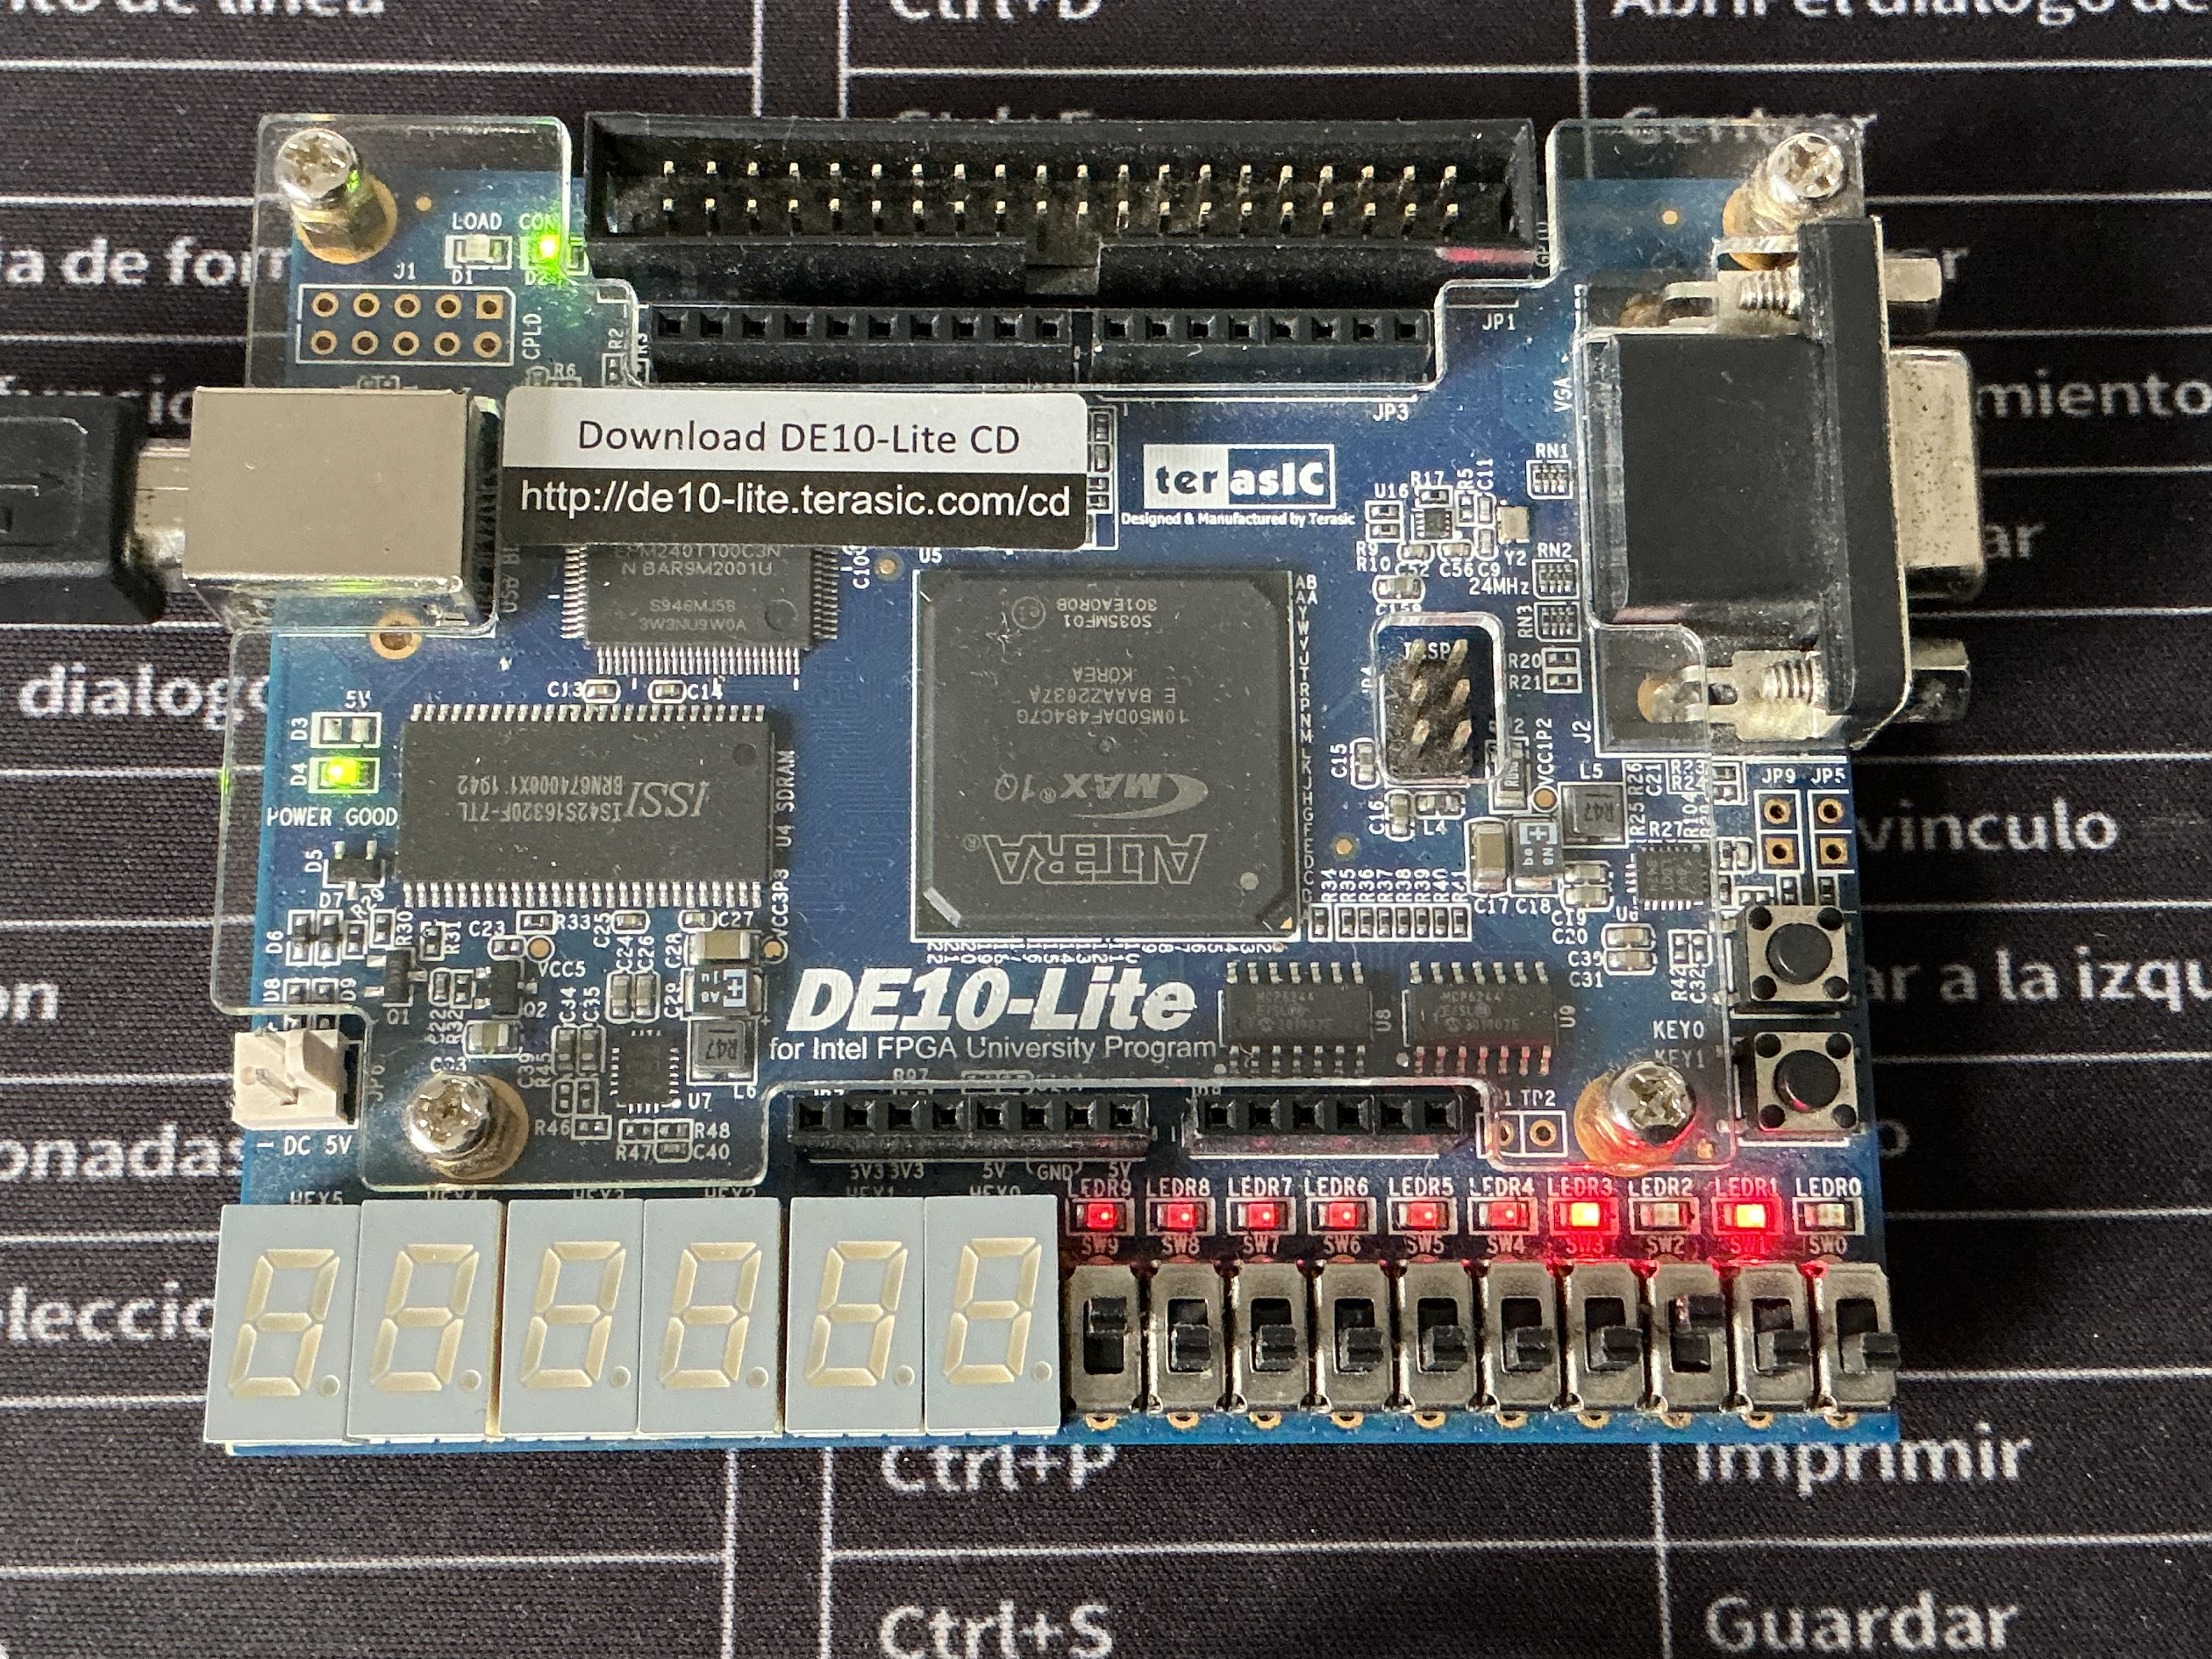
\includegraphics[width=\linewidth]{100.jpeg}
  \caption{\texttt{100}: salto de transformación.}
\end{subfigure}\hfill
\begin{subfigure}[b]{0.47\linewidth}
  \centering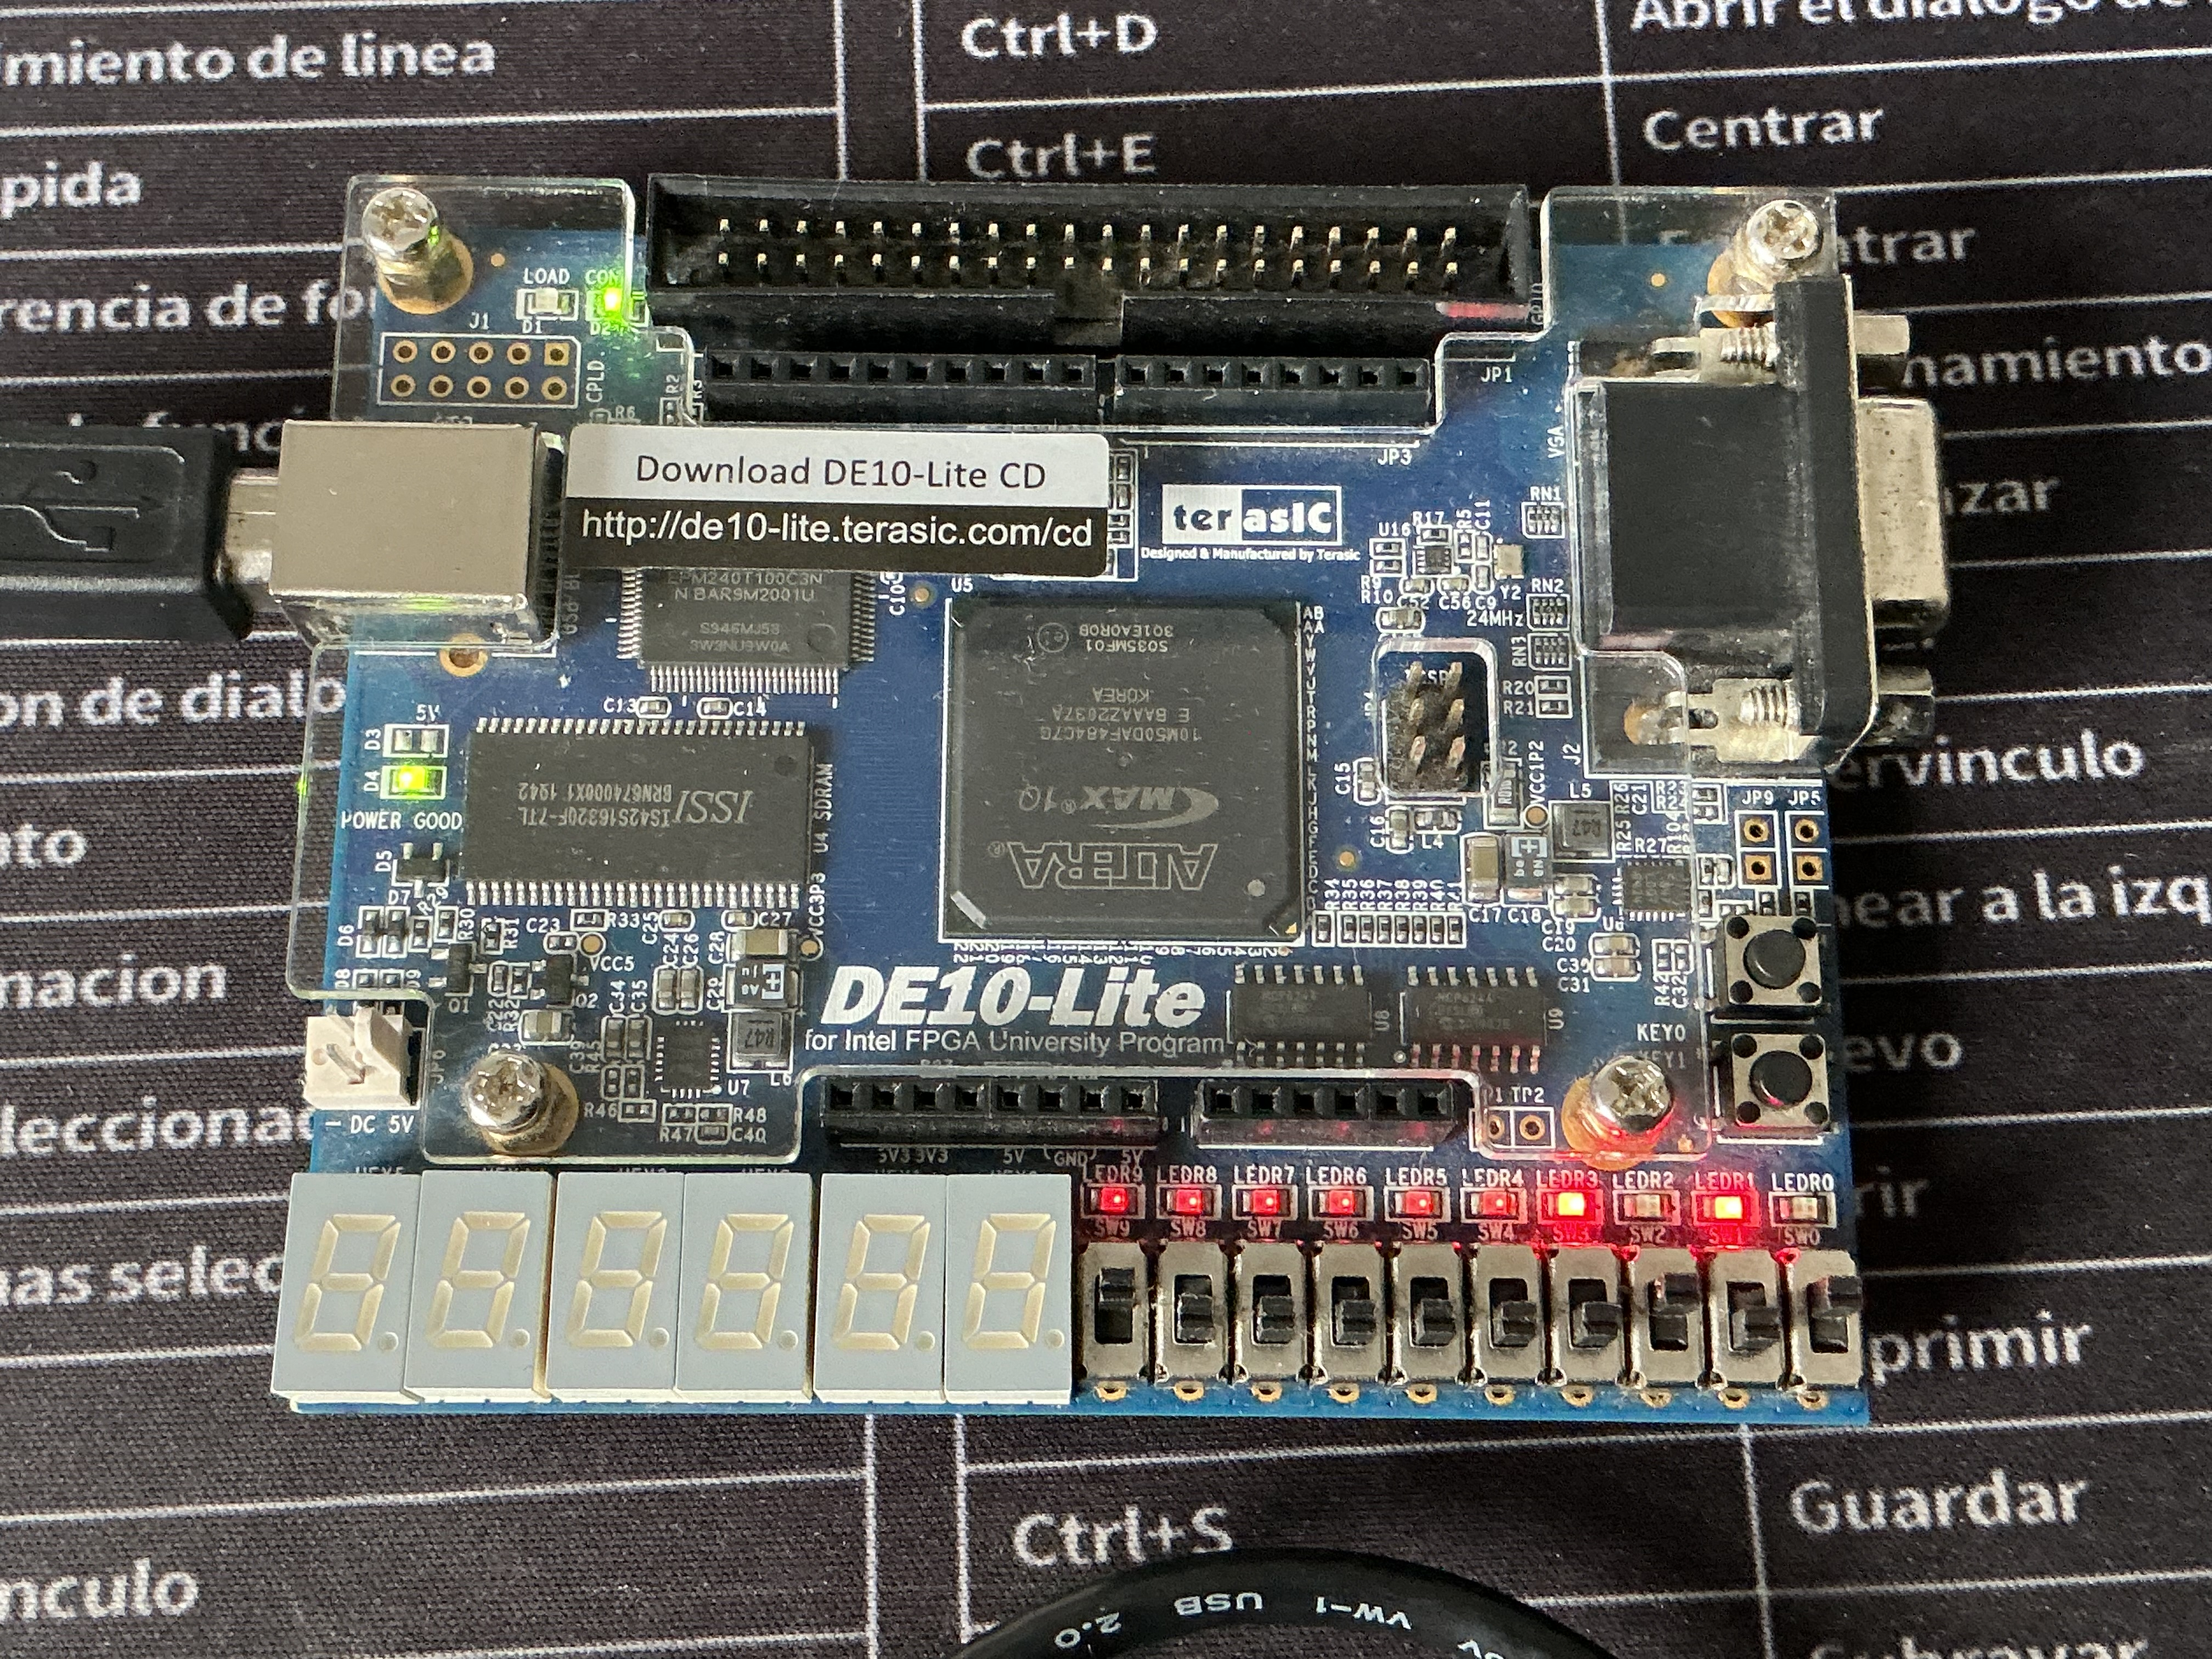
\includegraphics[width=\linewidth]{101.jpeg}
  \caption{\texttt{101}: salto de transformación.}
\end{subfigure}
\caption{Comprobación del registro $RT$ para $I_1I_0=10$.}
\label{fig:fpga-10}
\end{figure}

\begin{figure}[H]
\centering
\begin{subfigure}[b]{0.47\linewidth}
  \centering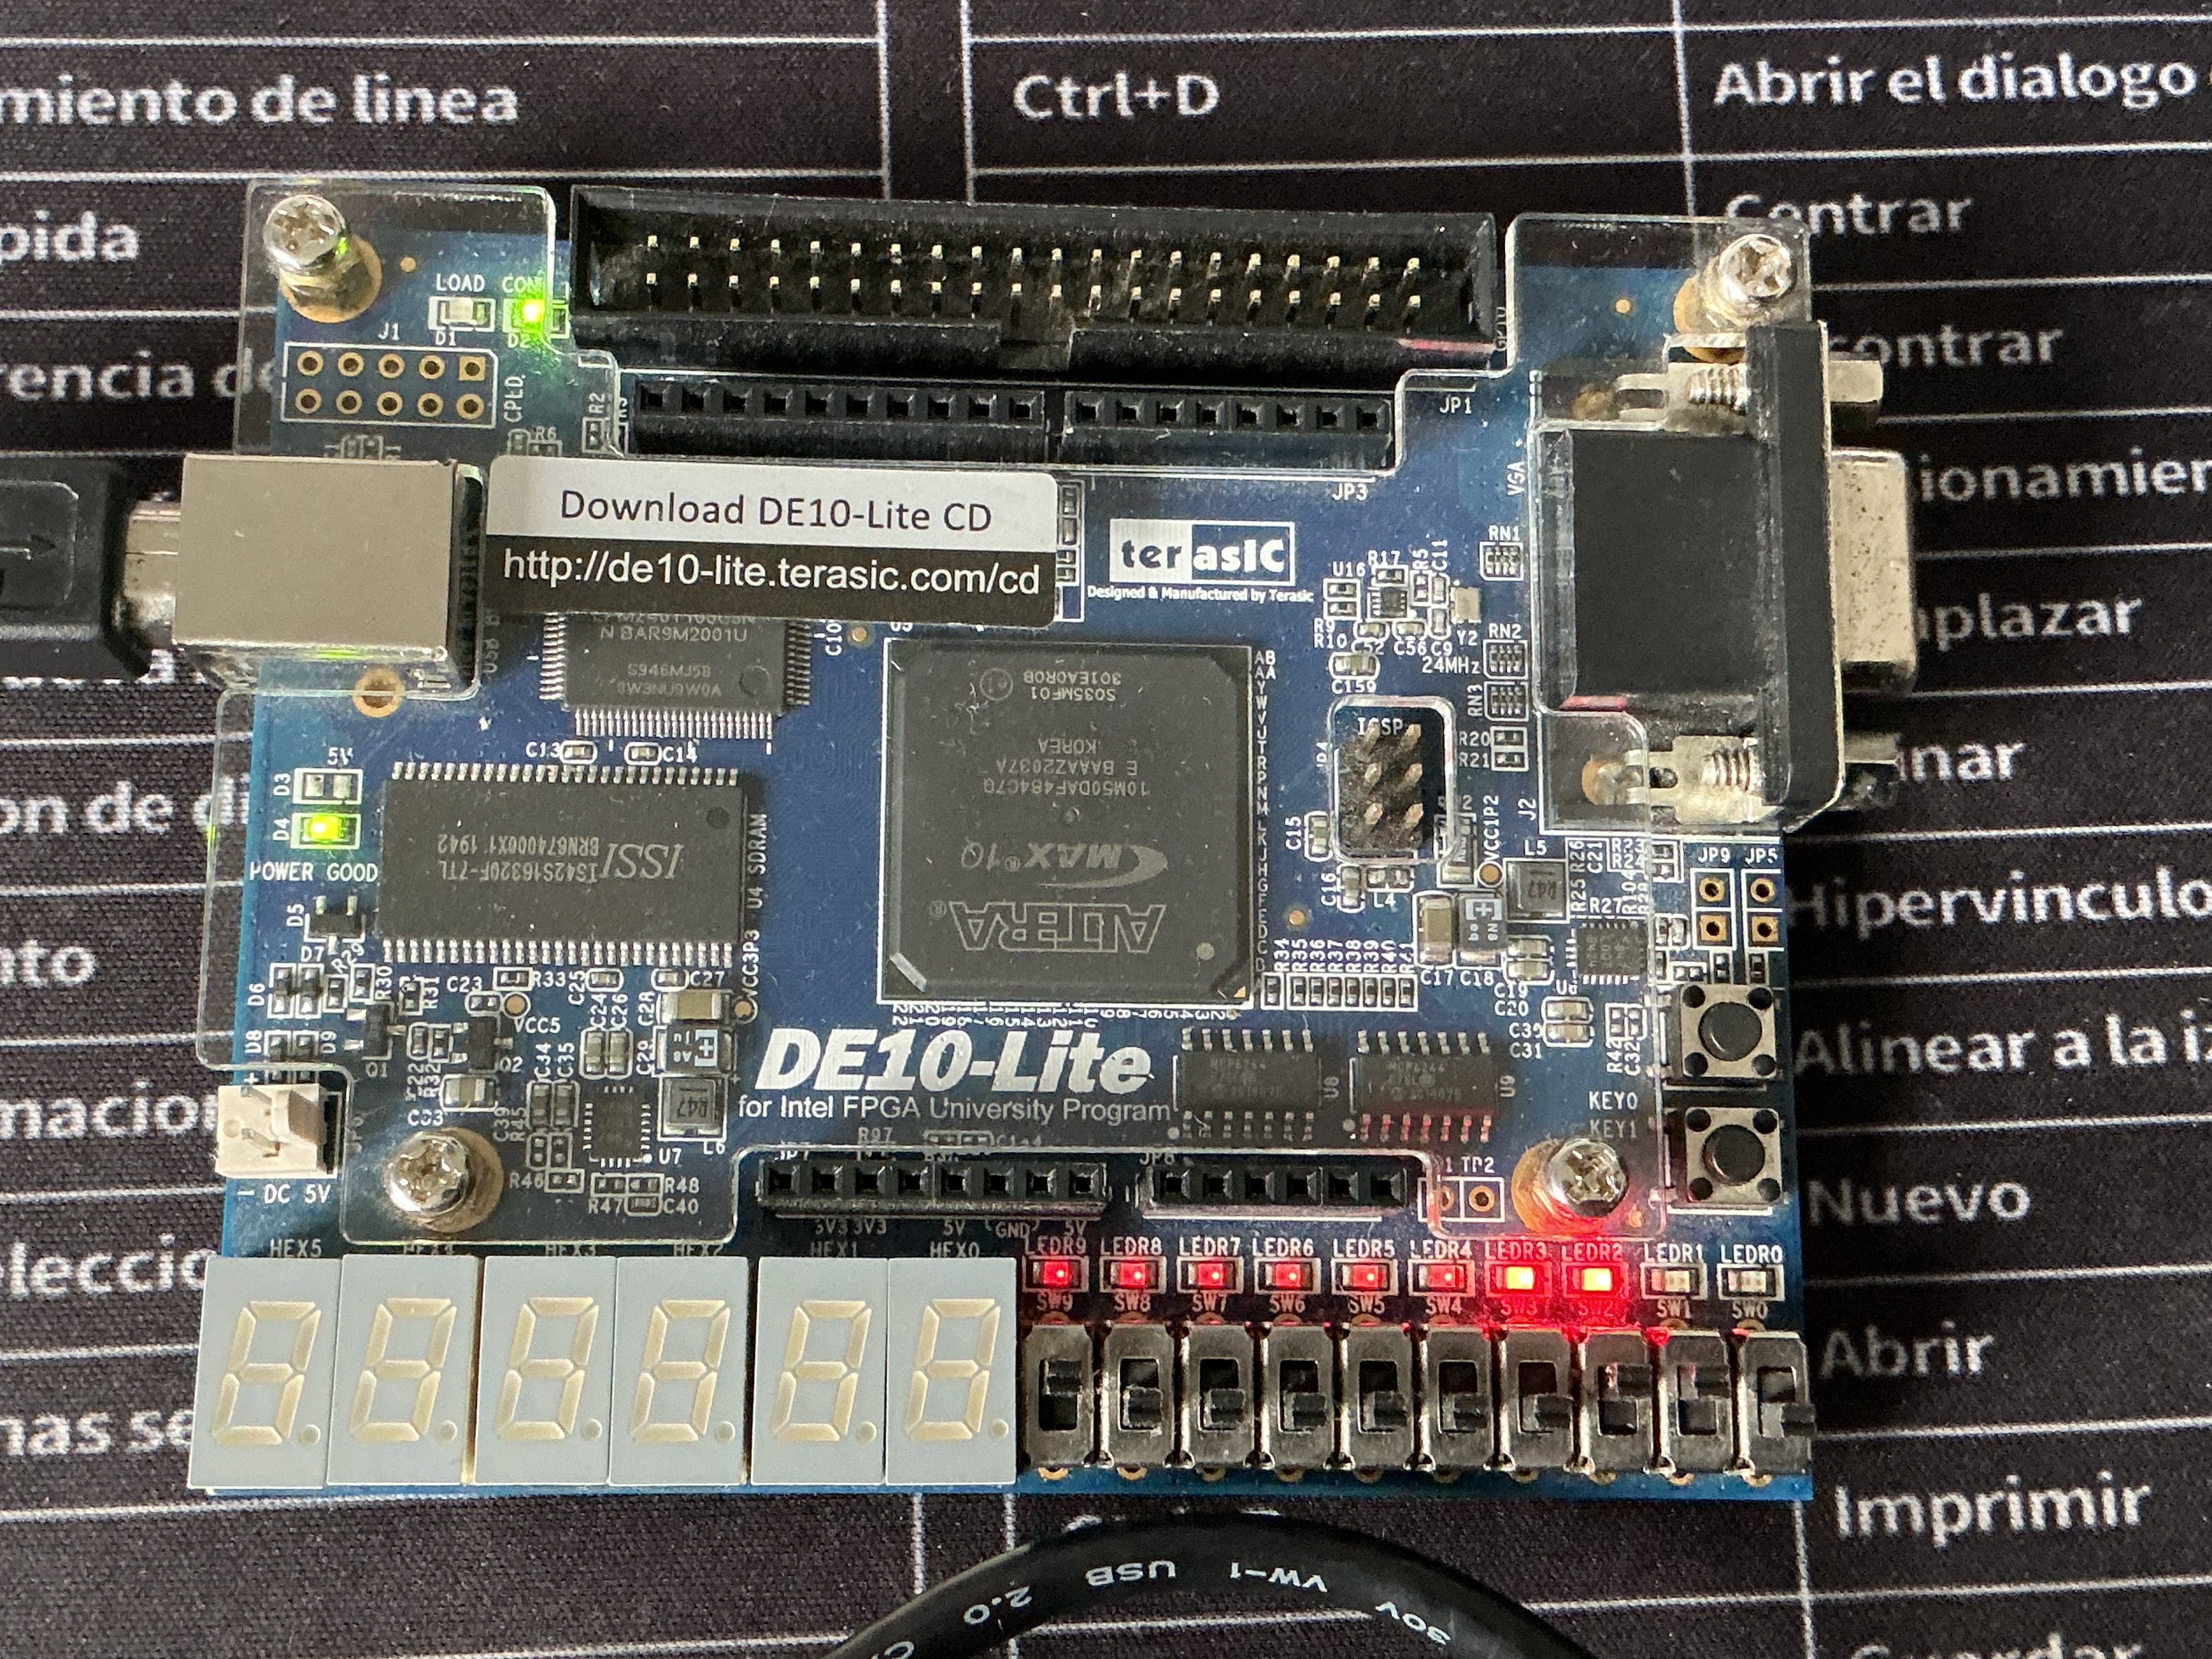
\includegraphics[width=\linewidth]{110.jpeg}
  \caption{\texttt{110}: salto de interrupción.}
\end{subfigure}\hfill
\begin{subfigure}[b]{0.47\linewidth}
  \centering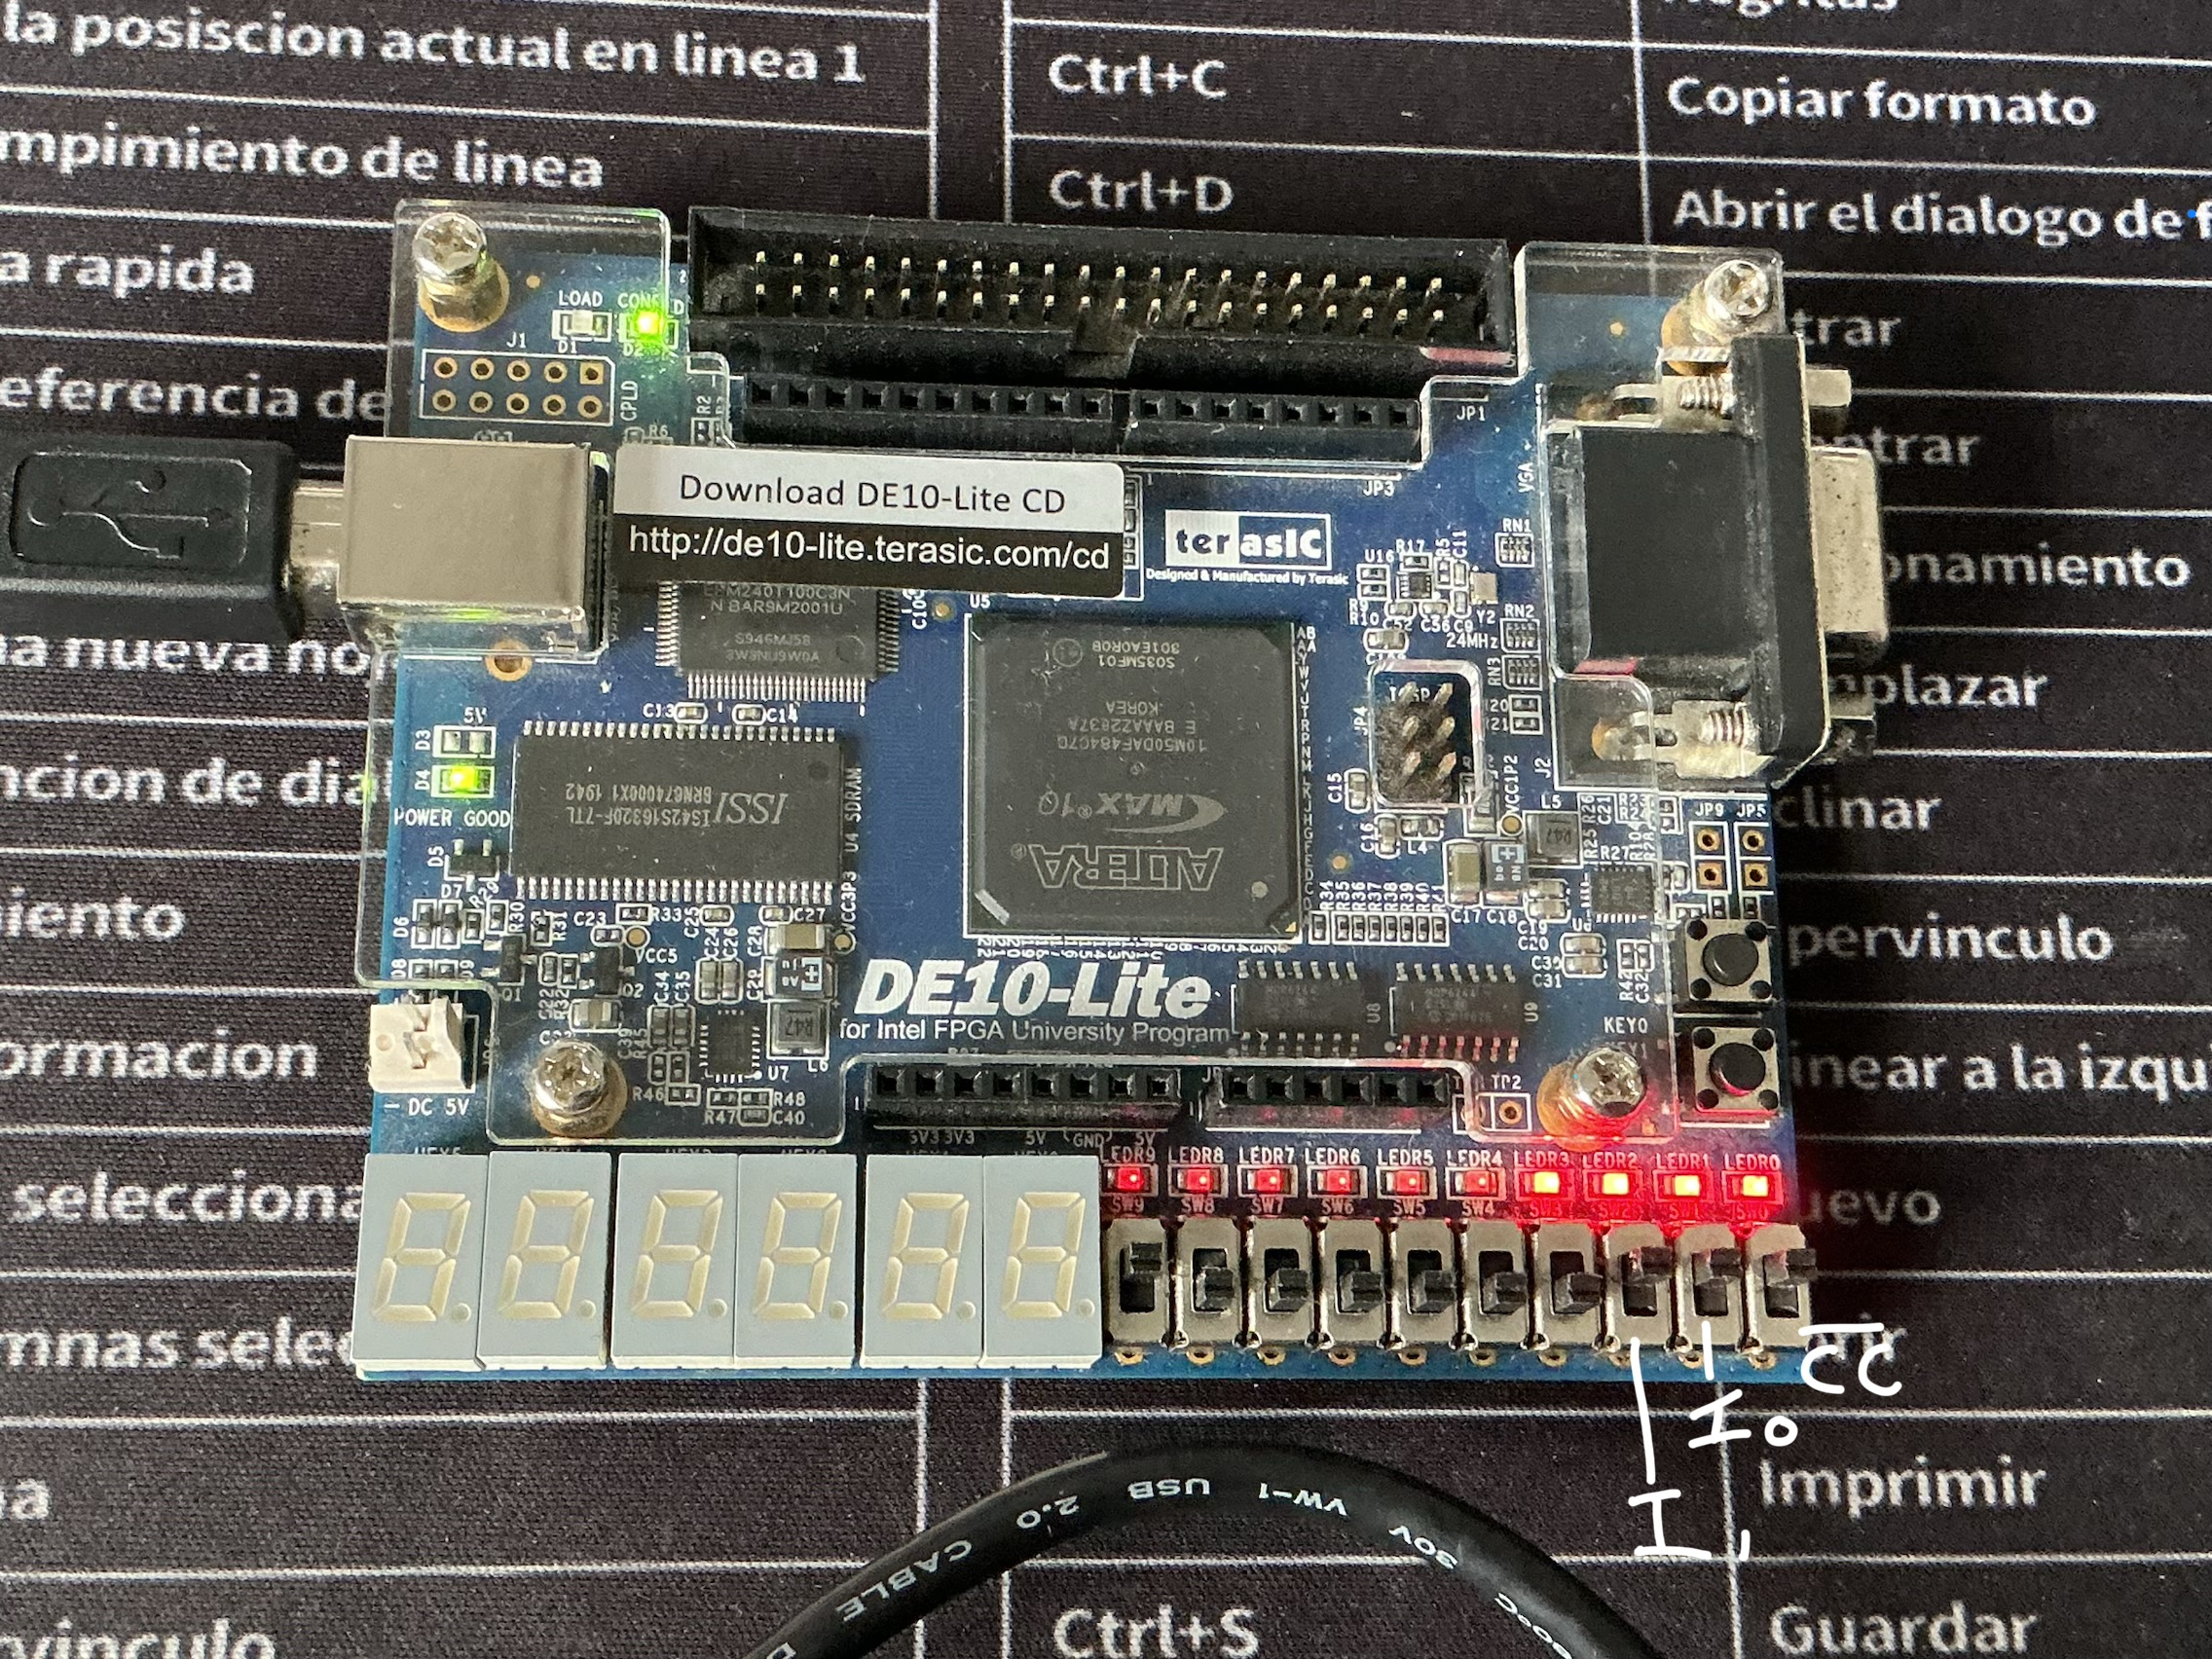
\includegraphics[width=\linewidth]{111.jpeg}
  \caption{\texttt{111}: avance continuo.}
\end{subfigure}
\caption{Comprobación del modo de interrupción para $I_1I_0=11$.}
\label{fig:fpga-11}
\end{figure}

La implementación física confirma que la siguiente microdirección sólo se registra en el pulso de reloj y que la lógica interna selecciona correctamente una de las cuatro fuentes. También se comprobó que el reinicio activo en bajo devuelve el contador de microprograma a \texttt{0000}, lo que permite iniciar cualquier secuencia desde una dirección conocida.

\clearpage
\section{Conclusión}

\paragraph{Percival Ulises Espinoza Matamoros.} A partir de la implementación del secuenciador básico comprendí cómo se obtiene la siguiente microdirección en una unidad de control microprogramada. La práctica permitió diferenciar el paso continuo, el salto condicional, el salto de transformación y el salto por interrupción, así como observar que todos ellos terminan actualizando el mismo registro $mPC$.

\paragraph{Oscar Iván Montiel Juárez.} El desarrollo de esta práctica permitió conocer la importancia del contador de microprograma y de la lógica de selección dentro de un procesador. Al conectar el incrementador, los registros de liga, transformación e interrupción con el multiplexor se pudo comprobar que una sola arquitectura puede generar distintos recorridos dependiendo de los bits de microinstrucción y de la condición de control. La simulación y la tarjeta permitieron verificar cada caso de manera visual.

\paragraph{Amy Valentina Veraza García.} La práctica ayudó a reforzar la relación entre las microinstrucciones y el funcionamiento de la ruta de control. Al probar el circuito en la DE10-Lite fue posible observar los cambios de dirección en cada pulso de reloj y comprobar que el valor de $CC$ sólo afecta a los tipos de salto que requieren una decisión.

\end{document}
